\documentclass[11pt,a4paper]{article}

% --- Packages ---
\usepackage[utf8]{inputenc}
\usepackage[T1]{fontenc}
\usepackage{amsmath,amssymb,amsfonts}
\usepackage{graphicx}
\usepackage{booktabs}
\usepackage{hyperref}
\usepackage[numbers,sort&compress]{natbib}
\usepackage[margin=1in]{geometry}
\usepackage{algorithm}
\usepackage{algorithmic}
\usepackage{multirow}
\usepackage{caption}
\usepackage{subcaption}
\usepackage{xcolor}
\usepackage{float}

% --- Hyperref setup ---
\hypersetup{
    colorlinks=true,
    linkcolor=blue,
    citecolor=blue,
    urlcolor=blue
}

% --- Custom commands ---
\newcommand{\R}{\mathbb{R}}
\newcommand{\E}{\mathbb{E}}
\newcommand{\Prob}{\mathbb{P}}

\title{Continuous Gaussian Hidden Markov Models for Equity and Volatility Index Dynamics:\\A Baum-Welch Approach Without Jump Augmentation, with Cross-Asset SIM and Copula Extensions}

\author{
    Abdulrahman Alswaidan\thanks{Cornell University, Robert Frederick Smith School of Chemical and Biomolecular Engineering, Ithaca, NY, USA. Email: \texttt{aa2725@cornell.edu}.}
    \and
    Cade Jin\thanks{Cornell University, Ithaca, NY, USA. Email: \texttt{cj383@cornell.edu}.}
    \and
    Jeffrey D.\ Varner\thanks{Cornell University, Robert Frederick Smith School of Chemical and Biomolecular Engineering, Ithaca, NY, USA. Email: \texttt{jdv27@cornell.edu}.}
}

\date{\today}

\begin{document}

\maketitle

% ========================================================================================= %
\begin{abstract}
We present a continuous hidden Markov model (CHMM) with Gaussian emissions trained via the Baum-Welch (Expectation-Maximization) algorithm for generating synthetic financial time series that preserve the canonical stylized facts of asset returns.
Unlike the discrete-state framework of \citet{alswaidan2026hybrid}, which requires Laplace quantile binning and a Poisson jump-duration mechanism to achieve volatility clustering, we show that the continuous model at a single moderate state resolution ($K = 18$, selected from a sweep over $K \in \{3, 6, 9, 12, 15, 18, 21\}$) reproduces all three stylized facts (heavy tails, negligible linear autocorrelation, and persistent volatility clustering) without jump augmentation, thereby eliminating two tunable hyperparameters ($\epsilon$, $\lambda$) and the discretization step entirely.

We benchmark the CHMM against six alternative generators on ten years of daily S\&P~500 ETF (SPY) data: bootstrap resampling, Gaussian and Laplace i.i.d.\ generators, the \emph{discrete} HMM of \citet{alswaidan2026hybrid} in both no-jump (NJ) and Poisson-jump (WJ, $\epsilon = 0.01$, $\lambda = 3$) variants, and GARCH(1,1).
Evaluation uses seven complementary metrics (Kolmogorov--Smirnov and Anderson--Darling pass rates, excess kurtosis, autocorrelation function mean absolute error, Wasserstein-1 and Hellinger distances, and quantile coverage) applied to 1{,}000 simulated paths in both in-sample (2014--2024) and out-of-sample (2025) windows.
Cross-asset generalization to NVDA, JNJ, JPM, AAPL, and QQQ confirms adaptability to diverse risk profiles.

To move from univariate to multi-asset generation we extend the framework with two cross-asset dependence models that preserve each asset's fitted CHMM marginal: a Single Index Model (SIM) factor construction with SPY as the market engine, and Gaussian / Student-t copulas fitted to rank-based correlation and simulated via rank reordering.
On six SPY-member assets the copula-based dependence models substantially outperform the SIM factor baseline on per-asset distributional accuracy (median in-sample KS pass rate 98.0\% for both copulas versus 83.8\% for SIM) while also delivering closer correlation-matrix reproduction (off-diagonal MAE 0.027 for Student-t, 0.031 for Gaussian, and 0.078 for SIM).
The Student-t copula's profile MLE selected $\nu^{*} = 6$ degrees of freedom, indicating economically meaningful joint tail dependence.

We further extend the framework to CBOE Volatility Index (VIX) and VXX log returns, demonstrating that the CHMM captures the distinct statistical properties of volatility indices (including stronger mean reversion, positive skewness, and pronounced regime structure).
The VIX regime decomposition provides a natural bridge to option pricing: median VIX levels per decoded regime define a volatility map that drives regime-switching geometric Brownian motion paths.
A parametric stochastic-volatility comparison against the resulting implied volatility surface is the subject of companion work and is deliberately outside the scope of this paper.

\bigskip\noindent
\textbf{Keywords:} Continuous Hidden Markov Model, Baum-Welch Algorithm, Stylized Facts, Volatility Clustering, Regime-Switching, Synthetic Financial Data, Single Index Model, Copula Dependence, Cross-Asset Simulation, VIX.
\end{abstract}

% ========================================================================================= %
\section{Introduction}
\label{sec:introduction}
\input{sections/introduction_v4}

\section{Related Work}
\label{sec:related}
Research on reproducing the canonical stylized facts of financial markets spans parametric return models, latent-state frameworks, multi-asset dependence modeling, and deep generative approaches.
This section reviews the key developments that motivate the present work, with particular attention to the Gaussian HMM limitation identified by \citet{ryden1998stylized} that our results challenge, and to the cross-asset dependence models that we use in our multi-asset extension.

\subsection{Stylized Facts of Asset Returns}

The Black--Scholes--Merton framework \cite{black1973pricing} assumes that log-returns are independently and identically distributed (i.i.d.) Gaussian random variables.
This assumption, while analytically convenient, is contradicted by a large body of empirical evidence accumulated over six decades.
\citet{mandelbrot1963variation} demonstrated that speculative price changes exhibit heavy tails (leptokurtosis), with extreme returns occurring far more frequently than a Gaussian model predicts.
\citet{fama1970efficient} confirmed negligible linear autocorrelation in raw returns, consistent with informational efficiency, but this does not imply independence: nonlinear dependence persists in the form of volatility clustering.
\citet{schwert1989does} documented that the autocorrelation of absolute returns decays slowly, often following a hyperbolic rather than exponential pattern, providing the empirical signature of clustered volatility.

\citet{cont2001empirical} systematized these observations into a canonical set of stylized facts that hold across asset classes, geographic markets, and sampling frequencies:
\begin{enumerate}
    \item \textit{Heavy tails}: the marginal distribution of returns exhibits positive excess kurtosis, with power-law tail decay.
    \item \textit{Absence of linear autocorrelation}: raw returns are approximately uncorrelated, consistent with market efficiency.
    \item \textit{Volatility clustering}: the autocorrelation of absolute (or squared) returns is positive and decays slowly, indicating that large price movements tend to be followed by large movements of either sign.
\end{enumerate}
Any generative model for financial time series must simultaneously reproduce all three facts to be considered statistically faithful.
Failure to capture even one, as we will show for the Gaussian i.i.d.\ generator (distributional failure) and GARCH(1,1) (distributional failure despite temporal fidelity), renders the synthetic data inadequate for downstream applications such as risk measurement and portfolio backtesting.

\subsection{Parametric Volatility Models}

The ARCH model of \citet{engle1982autoregressive} introduced conditional heteroscedasticity into time series econometrics, modeling the variance of returns as a function of past squared residuals.
The generalized ARCH (GARCH) extension of \citet{bollerslev1986generalized} added lagged conditional variance, producing the workhorse GARCH(1,1) specification
\begin{equation}
    \sigma_t^2 = \omega + \alpha\, r_{t-1}^2 + \beta\, \sigma_{t-1}^2
    \label{eq:garch_lit}
\end{equation}
where $\alpha + \beta < 1$ ensures stationarity.
The single-decay parameter $\beta$ directly controls the persistence of the conditional variance process, producing exponential ACF decay that closely approximates the empirical pattern when $\alpha + \beta$ is near unity.
However, GARCH models assume a unimodal innovation distribution and cannot represent discrete market regimes.
As we demonstrate empirically, this unimodal assumption leads to catastrophic distributional failure: GARCH(1,1) achieves only 13\% KS pass rate despite matching the observed ACF-MAE almost exactly (0.047 vs.\ 0.048 observed).

Parametric stochastic-volatility models treat log-variance as a latent diffusion, but parameter estimation requires computationally intensive methods such as particle filtering or Markov-chain Monte Carlo, and they are orthogonal to the synthetic-data-generation problem addressed here.

Jump-diffusion models \cite{merton1976option, kou2002jump} augment the geometric Brownian motion with Poisson-driven jumps in the price level, producing heavy-tailed marginal distributions.
\citet{merton1976option} used Gaussian jump sizes, while \citet{kou2002jump} introduced double-exponential jumps to capture the asymmetry between upside and downside tail risk.
These models generate heavy tails but lack a mechanism for volatility persistence: after a jump event, the volatility returns immediately to its baseline level, failing to reproduce the clustering phenomenon.

\subsection{Hidden Markov Models and the Ryd\'{e}n et al.\ Limitation}

\citet{hamilton1989new} introduced the Markov-switching model to economics, demonstrating that U.S.\ GNP growth is well described by a two-state regime-switching process.
The model posits a discrete latent state $S_t$ that evolves as a first-order Markov chain, with the observable variable drawn from a state-dependent distribution.
HMMs have since been applied to financial time series for regime identification \cite{kim1999has}, volatility estimation \cite{rossi2006volatility}, and trading strategy design \cite{nguyen2018hidden}.

The seminal evaluation of HMMs against stylized facts is due to \citet{ryden1998stylized}, who fitted Gaussian-emission HMMs with $K = 2$ and $K = 3$ states to daily Swedish equity returns.
They established three key findings.
First, HMMs produce heavy-tailed marginal distributions through the Gaussian mixture mechanism, even though each component is thin-tailed.
Second, HMMs produce negligible linear autocorrelation in returns, consistent with the observed stylized fact.
Third, HMMs \emph{fail} to reproduce the slow decay of the ACF of absolute returns (volatility clustering).
The third finding follows from a structural property of Markov chains: the sojourn time in any state follows a geometric distribution, which implies exponential decay of the ACF.
For $K = 2$--$3$ states, the exponential decay is too fast to approximate the hyperbolic-like persistence observed empirically.
This result has been widely cited as a fundamental limitation of standard HMMs for financial modeling.

\citet{bulla2006stylized} proposed hidden semi-Markov models (HSMMs) as a remedy.
HSMMs replace the geometric sojourn-time distribution with flexible parametric alternatives such as negative binomial or log-series, allowing arbitrarily slow ACF decay.
They demonstrated that HSMMs with $K = 2$--$4$ states and negative-binomial sojourn distributions successfully reproduce all three stylized facts, confirming that the Ryd\'{e}n limitation is fundamentally about the sojourn-time distribution, not the HMM framework itself.

The present work offers an alternative resolution: rather than modifying the sojourn-time distribution, we increase the state resolution.
With $K \geq 3$ states and quantile-based initialization, the Baum-Welch algorithm learns a transition matrix where high-volatility states exhibit sufficient self-transition probability (diagonal dominance) to sustain persistence.
The resulting mixture of $K$ geometric sojourn-time distributions, each with a different rate parameter, can approximate slow ACF decay, effectively achieving an HSMM-like effect within the standard HMM framework.
This insight has not been explored in the prior literature, likely because \citet{ryden1998stylized} only tested $K = 2$--$3$ and subsequent work adopted the HSMM path.

\subsection{Discrete HMM with Jump Augmentation}

\citet{alswaidan2026hybrid} addressed the Ryd\'{e}n limitation through a different mechanism: a Poisson jump-duration process that forces the model to dwell in tail states for durations drawn from a Poisson distribution, overriding the geometric sojourn time.
Their discrete framework used Laplace quantile binning to partition continuous observations into categorical states, estimated the transition matrix by direct frequency counting, and employed Student-$t$ within-bin emission distributions.
The jump mechanism introduced two hyperparameters ($\epsilon$ for jump probability, $\lambda$ for mean duration) calibrated via grid search.
The framework achieved 91--95\% KS pass rates across 424 US equities and partially reproduced volatility clustering.

The present work eliminates all three sources of complexity introduced by the discrete framework.
First, continuous Gaussian emissions replace Laplace quantile binning, removing discretization artifacts.
Second, the Baum-Welch algorithm jointly learns emissions and transitions, replacing frequency counting.
Third, no jump mechanism is needed at moderate $K$, removing two hyperparameters and the grid search entirely.

\subsection{Cross-Asset Dependence Models}
\label{sec:related_dep}

Generating jointly plausible multi-asset paths is a separate problem from univariate fidelity.
Two approaches dominate the quantitative finance literature.

\textit{Single Index Model (SIM).}
\citet{sharpe1963simplified} proposed a one-factor decomposition in which each asset's return is an affine function of a single market factor plus an idiosyncratic residual, $G_{i,t} = \alpha_i + \beta_i G_{M,t} + \eta_{i,t}$.
The SIM is parsimonious, analytically tractable, and is the workhorse reduction behind the mean-variance portfolio construction of \citet{markowitz1952portfolio}.
Its main limitations for synthetic data generation are that (i) the linear affine map distorts each asset's marginal distribution, so per-asset distributional fidelity degrades relative to the stand-alone marginal model, and (ii) it imposes a rank-one correlation structure in which all cross-asset dependence is mediated by the market factor.

\textit{Copulas.}
Sklar's theorem \cite{sklar1959fonctions, nelsen2006introduction} states that any joint cumulative distribution $H$ with continuous marginals $F_1, \dots, F_d$ factors uniquely as
\begin{equation}
    H(g_1, \dots, g_d) = C\bigl(F_1(g_1), \dots, F_d(g_d)\bigr),
\end{equation}
where the copula $C : [0,1]^d \to [0,1]$ is a multivariate distribution with uniform margins.
This factorization allows the joint distribution to be assembled from arbitrary per-asset marginals and any dependence structure $C$.
Within quantitative finance, the Gaussian and Student-t copulas \cite{demarta2005tcopula, mcneil2015quantitative} are standard choices because they admit analytic densities, are parameterized by a correlation matrix, and (for the Student-t copula) admit non-zero symmetric tail dependence controlled by the degrees-of-freedom parameter $\nu$.
Simulation via rank reordering \cite{iman1982distribution} exploits the uniqueness of Sklar's decomposition to inject the copula-sampled dependence structure onto independently simulated marginals without distorting any marginal distribution.

We adopt the copula construction of \cite{mcneil2015quantitative} for our cross-asset extension: per-asset CHMM simulations provide the marginals, Kendall's $\tau$ provides a robust rank-based correlation estimator, and the Student-t copula's degrees of freedom are selected by profile maximum likelihood.
The empirical ordering we report in Section~\ref{sec:cross_asset} (copulas ahead of SIM on both per-asset KS and cross-asset correlation reproduction) matches the ordering reported by \citet{alswaidan2026hybrid} for the discrete HMM marginals, suggesting that the copula advantage is intrinsic to the rank-reordering construction rather than specific to the marginal model.

\subsection{Deep Generative Models}

Deep generative models have attracted growing interest for financial time series synthesis.
\citet{takahashi2019modeling} applied generative adversarial networks (GANs) to stock return generation, finding that GAN-produced sequences visually resembled financial data but failed to reproduce ACF structure (the same volatility-clustering limitation as low-$K$ HMMs).
\citet{kwon2024can} systematically evaluated several GAN architectures against the Cont stylized facts and confirmed that volatility clustering remained the most difficult property to capture, unless the architecture was specifically designed to encode temporal dependence (for example, through recurrent discriminators).

\citet{alswaidan2026hybrid} benchmarked a GRU-based generator against HMM variants and found that it closed 83\% of the ACF-MAE gap relative to the HMM, but suffered variance collapse (0.6\% KS pass rate), indicating that distributional fidelity and temporal structure remain in tension for neural approaches.
The present study focuses on the parametric HMM approach, which offers interpretability (each state corresponds to a named market regime), computational efficiency ($O(TK^2)$ per Baum-Welch iteration), and guaranteed convergence (EM monotonicity), advantages that complement the flexibility of deep generative methods.

\subsection{Quality Assessment for Synthetic Time Series}

\citet{stenger2024thinking} surveyed the quality assessment landscape for synthetic time series, organizing evaluation metrics into distributional fidelity, temporal fidelity, and downstream utility categories.
Our seven-metric evaluation framework (KS and AD pass rates, excess kurtosis, ACF-MAE, Wasserstein-1, Hellinger distance, and quantile coverage) spans the first two categories, providing a comprehensive assessment that avoids reliance on any single metric.
As we will demonstrate, no single model dominates all seven metrics, and the choice of generator depends on which dimension of fidelity is prioritized.
\citet{assefa2020generating} made a complementary argument in the specific context of financial data, emphasizing that synthetic generators should be evaluated on their ability to preserve statistical properties relevant to the intended downstream application.


\section{Methods}
\label{sec:methods}
\subsection{Data}
\label{sec:data}

The empirical foundation of this study is a dataset of 424 United States-listed equities and exchange-traded funds spanning ten years of daily trading data (January~3, 2014 to December~31, 2024).
We focus the primary single-asset analysis on the SPDR S\&P~500 ETF Trust (SPY), which tracks the S\&P~500 index and is the most liquid equity ETF by trading volume.
The data include daily open, high, low, and close prices along with volume and volume-weighted average price (VWAP) metrics, sourced from standard financial data providers.
The in-sample (IS) dataset comprises $T_{\text{IS}} = 2{,}766$ trading days.
A subsequent $T_{\text{OoS}} = 219$ trading days in 2025 are reserved as a held-out out-of-sample (OoS) test set to evaluate generalization.

Cross-asset generalization is assessed on five additional tickers spanning distinct risk profiles: NVDA (NVIDIA Corporation; high-beta technology), JNJ (Johnson \& Johnson; low-beta healthcare), JPM (JPMorgan Chase \& Co.; moderate-beta financials), AAPL (Apple Inc.; large-cap consumer technology), and QQQ (Invesco QQQ Trust; Nasdaq-100 ETF).
For the univariate fidelity evaluation each asset is fitted independently using the same training/test split.
For the cross-asset extension of Section~\ref{sec:cross_asset_methods} we additionally stack the six-asset in-sample return matrix $\mathbf{R}_{\text{IS}} \in \mathbb{R}^{T_{\text{IS}} \times 6}$ to fit the cross-sectional dependence models.

To extend the framework beyond equity returns, we additionally apply it to the CBOE Volatility Index (VIX) \cite{whaley2009vix}, which measures the 30-day implied volatility of S\&P~500 options and is widely regarded as the market's ``fear gauge.''
VIX daily close prices spanning approximately 2006--2024 constitute the in-sample dataset, with 2025 data reserved for out-of-sample testing.
VIX log returns exhibit statistical properties that differ markedly from equity returns, including positive skewness (reflecting asymmetric volatility spikes), pronounced mean reversion, and extreme excess kurtosis, making it a challenging test case that probes the generality of the CHMM framework.

\subsection{Excess Growth Rate Calculation}
\label{sec:growth_rate}

We compute the annualized excess growth rate $G_{i,j}$ for ticker $i$ between trading days $j-1$ and $j$ given the equity price series $P_{i,j}$:
\begin{equation}
    G_{i,j} \equiv \frac{1}{\Delta t} \cdot \ln\!\left(\frac{P_{i,j}}{P_{i,j-1}}\right) - r_f
    \label{eq:growth_rate}
\end{equation}
where $\Delta t = 1/252$ (one trading day expressed in years) and $r_f$ is a constant risk-free rate set to zero throughout this study.
The resulting excess growth rate has units of year$^{-1}$ and is time-additive under continuous compounding.
The annualization by $1/\Delta t$ scales the daily log-returns to an annualized basis, producing values with magnitudes on the order of $\pm 2$ standard deviations for typical daily moves.

\subsection{Continuous Hidden Markov Model}
\label{sec:chmm_def}

We define the continuous hidden Markov model (CHMM) as the tuple $\mathcal{M} = (\mathcal{S}, \mathcal{O}, \mathbf{T}, \mathbf{B}, \boldsymbol{\pi})$ \cite{rabiner1986introduction}, where
\begin{itemize}
    \item $S_t \in \mathcal{S} = \{1, 2, \ldots, K\}$ is the hidden state at time $t$, representing the prevailing market regime;
    \item $\mathcal{O} \subseteq \mathbb{R}$ is the continuous observation space of excess growth rates;
    \item $\mathbf{T} \in \mathbb{R}^{K \times K}$ is the state transition probability matrix with entries $T_{ij} = \Prob(S_{t+1} = j \mid S_t = i)$, satisfying $\sum_{j=1}^{K} T_{ij} = 1$ for all $i$;
    \item $\mathbf{B} = \{(\mu_k, \sigma_k)\}_{k=1}^{K}$ specifies the Gaussian emission distributions, where $G_t \mid S_t = k \sim \mathcal{N}(\mu_k, \sigma_k^2)$;
    \item $\boldsymbol{\pi} = (\pi_1, \ldots, \pi_K)$ is the initial state distribution with $\pi_k = \Prob(S_1 = k)$.
\end{itemize}

The emission density for state $k$ is
\begin{equation}
    b_k(x) = \frac{1}{\sigma_k \sqrt{2\pi}} \exp\!\left(-\frac{(x - \mu_k)^2}{2\sigma_k^2}\right).
    \label{eq:emission}
\end{equation}

The marginal distribution of $G_t$ under the stationary regime is a $K$-component Gaussian mixture,
\begin{equation}
    f(x) = \sum_{k=1}^{K} \bar{\pi}_k \, b_k(x),
    \label{eq:mixture}
\end{equation}
where $\bar{\boldsymbol{\pi}}$ is the stationary distribution satisfying $\bar{\boldsymbol{\pi}} = \bar{\boldsymbol{\pi}} \mathbf{T}$.
This mixture structure is the mechanism by which HMMs produce heavy-tailed marginal distributions from thin-tailed Gaussian components: tail states with large $|\mu_k|$ or $\sigma_k$ contribute to the kurtosis of the mixture even though each component has zero excess kurtosis individually.

Unlike the discrete framework of \citet{alswaidan2026hybrid}, which discretizes observations into Laplace quantile bins and estimates $\mathbf{T}$ by frequency counting, we learn $\mathbf{T}$, $\{\mu_k\}_{k=1}^{K}$, $\{\sigma_k\}_{k=1}^{K}$, and $\boldsymbol{\pi}$ jointly from the continuous observations via the Baum-Welch algorithm described below.

\subsection{Baum-Welch (EM) Algorithm}
\label{sec:baum_welch}

The Baum-Welch algorithm \cite{baum1970maximization} is the standard expectation-maximization (EM) procedure for maximum likelihood estimation of HMM parameters.
Given a sequence of $T$ observations $O_{1:T} = (O_1, O_2, \ldots, O_T)$, the algorithm iterates between an E-step and an M-step until convergence.

\paragraph{E-Step: Forward-Backward in Log-Space.}
Define the forward variable
$\alpha_t(k) = \Prob(O_{1:t},\, S_t = k \mid \mathcal{M})$
and the backward variable
$\beta_t(k) = \Prob(O_{t+1:T} \mid S_t = k, \mathcal{M})$.
The recursions are
\begin{align}
    \log \alpha_1(k) &= \log \pi_k + \log b_k(O_1) \label{eq:forward_init} \\
    \log \alpha_t(j) &= \underset{i}{\text{logsumexp}}\!\left(\log \alpha_{t-1}(i) + \log T_{ij}\right) + \log b_j(O_t), \quad t = 2, \ldots, T \label{eq:forward} \\[6pt]
    \log \beta_T(k) &= 0 \label{eq:backward_init} \\
    \log \beta_t(i) &= \underset{j}{\text{logsumexp}}\!\left(\log T_{ij} + \log b_j(O_{t+1}) + \log \beta_{t+1}(j)\right), \quad t = T{-}1, \ldots, 1 \label{eq:backward}
\end{align}
where the logsumexp operation is defined as
\begin{equation}
    \underset{i}{\text{logsumexp}}(x_i) = x_{\max} + \log\!\left(\sum_{i} \exp(x_i - x_{\max})\right), \quad x_{\max} = \max_i\, x_i.
    \label{eq:logsumexp}
\end{equation}
All forward-backward computations are performed entirely in log-space to prevent the floating-point underflow that occurs when multiplying many small probabilities for long observation sequences \cite{bilmes1998gentle}.

The posterior state occupancy probability is
\begin{equation}
    \gamma_t(k) = \Prob(S_t = k \mid O_{1:T}, \mathcal{M}) = \frac{\alpha_t(k)\,\beta_t(k)}{\sum_{j=1}^{K} \alpha_t(j)\,\beta_t(j)}
    \label{eq:gamma}
\end{equation}
and the posterior transition probability is
\begin{equation}
    \xi_t(i,j) = \Prob(S_t = i, S_{t+1} = j \mid O_{1:T}, \mathcal{M}) = \frac{\alpha_t(i)\,T_{ij}\,b_j(O_{t+1})\,\beta_{t+1}(j)}{\sum_{m=1}^{K}\sum_{n=1}^{K}\alpha_t(m)\,T_{mn}\,b_n(O_{t+1})\,\beta_{t+1}(n)}.
    \label{eq:xi}
\end{equation}

\paragraph{M-Step: Parameter Re-Estimation.}
Given the posterior quantities $\gamma_t(k)$ and $\xi_t(i,j)$, the parameters are re-estimated as
\begin{align}
    \pi_k^{\text{new}} &= \gamma_1(k) \label{eq:pi_update} \\[4pt]
    \mu_k^{\text{new}} &= \frac{\displaystyle\sum_{t=1}^{T} \gamma_t(k) \cdot O_t}{\displaystyle\sum_{t=1}^{T} \gamma_t(k)} \label{eq:mu_update} \\[4pt]
    \left(\sigma_k^{\text{new}}\right)^2 &= \frac{\displaystyle\sum_{t=1}^{T} \gamma_t(k) \cdot (O_t - \mu_k^{\text{new}})^2}{\displaystyle\sum_{t=1}^{T} \gamma_t(k)} \label{eq:sigma_update} \\[4pt]
    T_{ij}^{\text{new}} &= \frac{\displaystyle\sum_{t=1}^{T-1} \xi_t(i,j)}{\displaystyle\sum_{t=1}^{T-1} \gamma_t(i)}. \label{eq:T_update}
\end{align}

\paragraph{Quantile-Based Initialization.}
The EM algorithm is well known to be sensitive to initial parameter values, with poor starting configurations leading to degenerate local optima where all states collapse to the global mean \cite{rabiner1986introduction}.
We employ a quantile-based initialization strategy: the $T$ observations are sorted in ascending order and partitioned into $K$ equal-sized chunks.
The sample mean and standard deviation of each chunk seed the corresponding state's emission parameters $(\mu_k^{(0)}, \sigma_k^{(0)})$.
The transition matrix $\mathbf{T}^{(0)}$ is initialized as $T_{ij}^{(0)} = 1/K$ for all $i, j$, and the initial distribution as $\pi_k^{(0)} = 1/K$.
This strategy ensures that the initial emission distributions span the full range of observations, with tail states initialized to capture extreme returns.

\paragraph{Convergence Criterion.}
The algorithm terminates when the absolute change in log-likelihood falls below a tolerance threshold,
\begin{equation}
    |\mathcal{L}^{(n)} - \mathcal{L}^{(n-1)}| < \text{tol},
    \label{eq:convergence}
\end{equation}
where $\mathcal{L}^{(n)} = \text{logsumexp}_{k}(\log \alpha_T^{(n)}(k))$ is the total log-likelihood at iteration $n$.
We set $\text{tol} = 10^{-4}$ and $\texttt{max\_iter} = 60$.
In practice, all models converged within 20--40 iterations (see Appendix~\ref{sec:supplemental} for convergence curves).

\paragraph{Simulation.}
Given a trained model $\mathcal{M}$, synthetic paths of length $T$ are generated by:
\begin{enumerate}
    \item Draw the initial state $S_1 \sim \text{Categorical}(\boldsymbol{\pi})$.
    \item For $t = 1, 2, \ldots, T$:
    \begin{enumerate}
        \item Emit $G_t \sim \mathcal{N}(\mu_{S_t}, \sigma_{S_t}^2)$.
        \item Transition to $S_{t+1} \sim \text{Categorical}(\mathbf{T}_{S_t, \cdot})$.
    \end{enumerate}
\end{enumerate}
No jump mechanism is applied.
The Markov transition dynamics alone govern the temporal evolution of the hidden state sequence.

\subsection{Discrete HMM Baseline (Prior Paper)}
\label{sec:discrete_hmm}

For a like-for-like comparison against the prior discrete framework of \citet{alswaidan2026hybrid}, we reproduce their discrete HMM exactly within the same evaluation pipeline.
Continuous returns are binned into $K_{\text{disc}} = 13$ quantile bins using the observed IS CDF.
Let $b(G_t) \in \{1, \dots, K_{\text{disc}}\}$ be the bin index for observation $G_t$; the transition matrix is estimated by frequency counting
\begin{equation}
    \hat{T}_{ij} \;=\; \frac{\#\{t : b(G_{t-1}) = i,\, b(G_t) = j\}}{\#\{t : b(G_{t-1}) = i\}},
    \label{eq:disc_T}
\end{equation}
and emissions are near-identity (each state emits its own bin index, with a small smoothing floor to avoid zero-probability entries).
Decoded bin indices are mapped back to continuous returns via per-bin centroids.
The ``no-jump'' (NJ) variant runs the chain with this transition matrix alone; the ``with-jumps'' (WJ) variant augments the dynamics with a Poisson jump-duration process at jump probability $\epsilon = 0.01$ and mean duration $\lambda = 3$, matching the grid-calibrated values reported by \citet{alswaidan2026hybrid}.
Because quantization onto $K_{\text{disc}} = 13$ bin centroids strips the within-bin tail mass from every simulated path, the discrete baselines provide a direct upper bound on how much of the CHMM's fidelity is attributable to continuous emissions rather than to regime structure per se.

\subsection{GARCH(1,1) Benchmark}
\label{sec:garch}

As the primary temporal benchmark, we fit a GARCH(1,1) model \cite{bollerslev1986generalized}:
\begin{align}
    G_t &= \mu + \sigma_t\, z_t, \quad z_t \overset{\text{i.i.d.}}{\sim} \mathcal{N}(0,1) \label{eq:garch_mean} \\
    \sigma_t^2 &= \omega + \alpha\, (G_{t-1} - \mu)^2 + \beta\, \sigma_{t-1}^2 \label{eq:garch_var}
\end{align}
where $\omega > 0$, $\alpha \geq 0$, $\beta \geq 0$, and $\alpha + \beta < 1$.
Parameters $(\mu, \omega, \alpha, \beta)$ are estimated by maximum likelihood via the Nelder--Mead simplex algorithm.
The GARCH model serves as a benchmark because it is the canonical parametric model for volatility dynamics: its single-decay parameter $\beta$ directly encodes exponential variance persistence, providing an upper bound on ACF reproduction for single-regime models.

\subsection{Baseline Generators}
\label{sec:baselines}

We include three additional generators as distributional reference points.

\paragraph{Bootstrap Resampling.}
Each synthetic path is constructed by sampling $T$ observations uniformly with replacement from the in-sample data.
The bootstrap preserves the exact empirical marginal distribution but destroys all temporal structure, serving as the non-parametric ceiling for distributional fidelity.

\paragraph{Gaussian i.i.d.\ Generator.}
Draws $G_t \overset{\text{i.i.d.}}{\sim} \mathcal{N}(\hat{\mu}, \hat{\sigma}^2)$, where $\hat{\mu}$ and $\hat{\sigma}$ are the sample mean and standard deviation of the in-sample data.
This generator serves as a negative control: it should fail all distributional tests due to its inability to produce heavy tails.

\paragraph{Laplace i.i.d.\ Generator.}
Draws $G_t \overset{\text{i.i.d.}}{\sim} \text{Laplace}(\hat{m}, \hat{b})$, where $\hat{m}$ is the sample median and $\hat{b}$ is the mean absolute deviation from the median.
The Laplace distribution produces moderate heavy tails (excess kurtosis $= 3$), providing an intermediate reference between the Gaussian and the heavy-tailed empirical distribution.

\subsection{Cross-Asset Dependence Models}
\label{sec:cross_asset_methods}

Let $\mathbf{R}_{\text{IS}} \in \mathbb{R}^{T \times d}$ denote the in-sample return matrix for $d$ assets, with columns indexed by $j = 1, \ldots, d$ and the market-factor column indexed by $m \in \{1, \ldots, d\}$.
Both constructions below preserve each asset's fitted CHMM marginal; they differ in how cross-asset dependence is imposed.

\paragraph{Single Index Model (SIM).}
Following \citet{sharpe1963simplified} and the multi-asset extension of \citet{alswaidan2026hybrid}, for each non-market asset $j \neq m$ we fit the affine factor equation
\begin{equation}
    G_{j,t} \;=\; \alpha_j \;+\; \beta_j\, G_{m,t} \;+\; \eta_{j,t}
    \label{eq:sim}
\end{equation}
by ordinary least squares on $\mathbf{R}_{\text{IS}}$, yielding estimates $\hat{\alpha}_j$, $\hat{\beta}_j$, per-asset residuals $\hat{\eta}_{j,1:T}$, and coefficient of determination $R^2_j$.
At simulation time, we draw $n_{\text{paths}}$ independent market-factor paths $G_{m,1:T}^{(p)}$ from the market-asset CHMM, resample idiosyncratic residuals $\hat{\eta}_{j,t}^{(p)}$ with replacement from the empirical residual vector, and compute
\begin{equation}
    \hat{G}_{j,t}^{(p)} \;=\; \hat{\alpha}_j \;+\; \hat{\beta}_j\, G_{m,t}^{(p)} \;+\; \hat{\eta}_{j,t}^{(p)}.
    \label{eq:sim_sim}
\end{equation}
The market column $G_{m,t}^{(p)}$ is itself a CHMM simulation, ensuring that the univariate fidelity of the market engine is inherited by the factor construction.
SIM is parsimonious (only $2(d-1)$ parameters plus the residual empirical distribution) but distorts each non-market marginal through the affine map in equation~\eqref{eq:sim_sim}.

\paragraph{Copulas.}
By Sklar's theorem \cite{sklar1959fonctions}, any joint cumulative distribution function $H(g_1, \dots, g_d)$ with continuous marginals $F_1, \dots, F_d$ decomposes uniquely as
\begin{equation}
    H(g_1, \dots, g_d) \;=\; C\bigl(F_1(g_1), \dots, F_d(g_d)\bigr),
    \label{eq:sklar}
\end{equation}
for some copula $C : [0,1]^d \to [0,1]$.
This decomposition underpins a principled approach to multi-asset simulation: fix each marginal $F_j$ to the per-asset CHMM and estimate only the copula $C$ from the cross-sectional co-movement.

\textit{Probability integral transform.}
We obtain pseudo-uniform observations via the nonparametric PIT $u_{j,t} = \text{rank}(g_{j,t}) / (T+1)$, which avoids the marginal misspecification risk of plugging in a parametric CDF.

\textit{Gaussian copula.}
The Gaussian copula $C_{\text{Ga}}(\mathbf{u}; \Sigma) = \Phi_d\bigl(\Phi^{-1}(u_1), \dots, \Phi^{-1}(u_d); \Sigma\bigr)$ is parameterized by the $d \times d$ correlation matrix $\Sigma$.
We estimate $\Sigma$ from the pairwise Kendall's $\tau$ matrix via the closed-form inversion $\rho_{ij} = \sin(\pi \tau_{ij} / 2)$ \cite{embrechts2002correlation, mcneil2015quantitative}, and project to the nearest positive semi-definite matrix with rescaled unit diagonal if needed.
The Gaussian copula has zero upper and lower tail dependence for all $\rho < 1$, which motivates the Student-t alternative.

\textit{Student-t copula.}
The Student-t copula $C_t(\mathbf{u}; \Sigma, \nu) = t_{d,\nu}\bigl(t_\nu^{-1}(u_1), \dots, t_\nu^{-1}(u_d); \Sigma\bigr)$ admits nonzero symmetric tail dependence $\lambda_U = \lambda_L = 2\, t_{\nu+1}\!\bigl(-\sqrt{(\nu+1)(1-\rho)/(1+\rho)}\bigr)$, controlled by $\nu$ \cite{demarta2005tcopula}.
We reuse the Kendall's-$\tau$ correlation estimate from the Gaussian copula and select $\nu$ by profile maximum likelihood over the discrete grid $\nu \in \{2, 3, 4, 5, 6, 8, 10, 15, 20, 30\}$.

\textit{Simulation via rank reordering.}
Following the rank-coupling construction of \citet{iman1982distribution}, cross-asset simulation proceeds path-by-path:
\begin{enumerate}
    \item Simulate $T$ independent paths $\tilde{g}_{j,1:T}^{(p)}$ from each asset's marginal CHMM, producing a matrix $\tilde{\mathbf{G}}^{(p)} \in \mathbb{R}^{T \times d}$.
    \item Sample $T$ copula variates $\mathbf{U}^{(p)} \in [0,1]^{T \times d}$ from $C$.
    \item For each column $j$, reorder $\tilde{g}_{j,1:T}^{(p)}$ so that its ranks match the ranks of $U_{j,1:T}^{(p)}$.
\end{enumerate}
Because reordering only permutes the simulated values, the marginal distribution of each column is preserved \emph{exactly}: the resulting $\hat{G}_{j,1:T}^{(p)}$ is a permutation of $\tilde{g}_{j,1:T}^{(p)}$, so every order statistic matches.
The copula, however, is imposed through the coupling of ranks across columns.

\subsection{Validation Metrics}
\label{sec:metrics}

We evaluate synthetic data quality using seven complementary metrics, following the framework of \cite{stenger2024thinking} and \cite{alswaidan2026hybrid}.
For each model, 1{,}000 independent paths of length $T$ are simulated (200 paths for the cross-asset extension, given the quadratic cost of the copula and SIM pipelines).
Each metric is computed per path and then aggregated.

\begin{enumerate}
    \item \textbf{KS pass rate (\%).}
    The proportion of simulated paths for which the two-sample Kolmogorov--Smirnov test \cite{kolmogorov1933, smirnov1948} fails to reject the null hypothesis of distributional equivalence with the reference data at significance level $\alpha = 0.05$.
    The KS statistic measures the maximum vertical distance between two empirical CDFs:
    \begin{equation}
        D_{n,m} = \sup_x |F_n(x) - G_m(x)|.
        \label{eq:ks}
    \end{equation}
    Higher pass rates indicate better distributional fidelity.

    \item \textbf{AD pass rate (\%).}
    The proportion of paths for which the two-sample Anderson--Darling test fails to reject at $\alpha = 0.05$.
    The AD test is more sensitive to tail discrepancies than the KS test, providing a complementary measure of distributional fit.

    \item \textbf{Excess kurtosis.}
    The mean simulated excess kurtosis across paths, compared to the observed value.
    Closer matching indicates better tail reproduction.
    Given the Gaussian emission assumption, the CHMM is expected to underestimate kurtosis relative to the true heavy-tailed distribution.

    \item \textbf{ACF-MAE.}
    The mean absolute error between the observed and mean simulated autocorrelation functions of absolute excess growth rates over $L = 252$ lags (one trading year),
    \begin{equation}
        \text{ACF-MAE} = \frac{1}{L} \sum_{\tau=1}^{L} \left|\hat{\rho}^{\text{obs}}_{|G|}(\tau) - \bar{\hat{\rho}}^{\,\text{sim}}_{|G|}(\tau)\right|,
        \label{eq:acf_mae}
    \end{equation}
    where $\bar{\hat{\rho}}^{\,\text{sim}}_{|G|}(\tau)$ is the mean simulated ACF at lag $\tau$.
    Lower values indicate better reproduction of volatility clustering.
    This is the critical metric for evaluating the Ryd\'{e}n et al.\ limitation.

    \item \textbf{Wasserstein-1 distance ($W_1$).}
    The mean absolute difference of sorted empirical quantiles, equivalent to the $L^1$ distance between the empirical CDFs \cite{glasserman2003monte},
    \begin{equation}
        W_1(F, G) = \int_0^1 |F^{-1}(u) - G^{-1}(u)|\,du,
        \label{eq:wasserstein}
    \end{equation}
    approximated by comparing sorted samples.
    Lower values indicate closer distributional match.

    \item \textbf{Hellinger distance ($H$).}
    A histogram-based distributional overlap distance in $[0,1]$,
    \begin{equation}
        H(P, Q) = \frac{1}{\sqrt{2}} \sqrt{\sum_{i=1}^{B} \left(\sqrt{p_i} - \sqrt{q_i}\right)^2},
        \label{eq:hellinger}
    \end{equation}
    where $p_i$ and $q_i$ are the bin probabilities of the observed and simulated histograms, respectively.
    $H = 0$ indicates identical distributions.

    \item \textbf{Quantile coverage (\%).}
    The fraction of 99 equally spaced quantiles (1st through 99th percentiles) of the observed distribution that fall within the $[5\text{th}, 95\text{th}]$ percentile envelope of the corresponding simulated quantiles across 1{,}000 paths.
    A coverage of 100\% indicates that the simulated distribution fully envelopes the observed distribution at all quantile levels, providing a calibration-style diagnostic of the simulation envelope.
\end{enumerate}

For the cross-asset extension we additionally track two cross-sectional metrics: the mean Frobenius norm $\|\hat{\Sigma}_{\text{sim}}^{(p)} - \hat{\Sigma}_{\text{obs}}\|_F$ and the mean absolute error of the off-diagonal Pearson correlations between simulated and observed return matrices, averaged over paths.
These quantify how faithfully each dependence model reproduces the cross-sectional correlation structure.

\subsection{Volatility Measures: VIX and VXX as Synthetic-Data Targets}
\label{sec:vix_methods}

To demonstrate that the same Baum-Welch pipeline generalizes beyond equities, we apply it to the two most widely tracked market volatility measures: the CBOE Volatility Index (VIX) and the iPath Series B S\&P 500 VIX Short-Term Futures ETN (VXX).
Both are treated as univariate return series and fitted independently.
The model specification, training, and simulation are identical to the equity pipeline of Sections~\ref{sec:chmm_def}--\ref{sec:baum_welch}; only the input series changes.
Daily log returns are computed as
\begin{equation}
    R_t^{\text{VIX}} = \ln\!\left(\frac{\text{VIX}_t}{\text{VIX}_{t-1}}\right),
    \qquad
    R_t^{\text{VXX}} = \ln\!\left(\frac{\text{VXX}_t}{\text{VXX}_{t-1}}\right).
    \label{eq:vix_returns}
\end{equation}

The same seven-metric evaluation from Section~\ref{sec:metrics} is applied path-by-path to 1{,}000 simulated return paths for each instrument.
The goal here is synthetic-data quality on volatility measures, which have positive skewness, pronounced mean reversion, and heavier-than-equity excess kurtosis; downstream risk applications that consume synthetic volatility paths (for example, VaR of volatility-sensitive portfolios or scenario stress tests) are direct consumers of this output.
Option pricing, implied-volatility-surface calibration, and stochastic-volatility benchmarking are explicitly out of scope and are not revisited in this paper.


\section{Empirical Study}
\label{sec:results}
\input{sections/results_v4}

\section{Discussion}
\label{sec:discussion}
\input{sections/discussion_v4}

\section{Conclusion}
\label{sec:conclusion}
\input{sections/conclusion_v4}

% ========================================================================================= %
\bibliographystyle{unsrtnat}
\bibliography{References_v4}

% ========================================================================================= %
\appendix
\section{Supplementary Material}
\label{sec:supplemental}
\subsection{Full State-Resolution Sensitivity Table}
\label{sec:sensitivity_table}

Table~\ref{tab:sensitivity} reports the full sweep summarized by Figure~\ref{fig:k_sweep_summary} in the main text.
Observed excess kurtosis is 7.71 IS and 6.24 OoS at all $K$.

\begin{table}[H]
\centering
\caption{State resolution sensitivity for SPY CHMM (1{,}000 paths, $\alpha = 0.05$). Every metric is computed on the identical simulation pipeline used for Table~\ref{tab:model_comparison} in the main text. Coverage was 100\% at every $K$ in both IS and OoS windows.}
\label{tab:sensitivity}
\small
\begin{tabular}{c cc cc cc c c c c}
\toprule
& \multicolumn{2}{c}{KS (\%)} & \multicolumn{2}{c}{AD (\%)} & \multicolumn{2}{c}{Kurtosis} & & & & \\
\cmidrule(lr){2-3} \cmidrule(lr){4-5} \cmidrule(lr){6-7}
$K$ & IS & OoS & IS & OoS & Obs & Sim & ACF-MAE & $W_1$ & $H$ & Cov (\%) \\
\midrule
3  & 89.7 & 92.3 & 81.4 & 83.2 & 7.71 & 3.94 & 0.0458 & 0.119 & 0.0790 & 100.0 \\
6  & 93.4 & 92.5 & 87.1 & 84.3 & 7.71 & 5.06 & 0.0490 & 0.106 & 0.0782 & 100.0 \\
9  & 92.9 & 91.9 & 83.3 & 84.1 & 7.71 & 3.70 & 0.0468 & 0.114 & 0.0779 & 100.0 \\
12 & 94.5 & 93.8 & 86.1 & 86.0 & 7.71 & 4.18 & 0.0479 & 0.109 & 0.0767 & 100.0 \\
15 & 94.2 & 93.4 & 88.5 & 85.8 & 7.71 & 4.52 & 0.0490 & 0.106 & 0.0766 & 100.0 \\
\textbf{18} & \textbf{95.2} & \textbf{95.6} & \textbf{88.4} & \textbf{90.0} & 7.71 & \textbf{5.11} & 0.0502 & \textbf{0.102} & 0.0771 & 100.0 \\
21 & 94.7 & 95.4 & 88.3 & 88.1 & 7.71 & 4.71 & 0.0505 & 0.103 & 0.0774 & 100.0 \\
\bottomrule
\end{tabular}
\end{table}

\subsection{Baum-Welch Convergence}
\label{sec:convergence}

Figure~\ref{fig:convergence_all} shows the Baum-Welch convergence curves for representative state resolutions.
All models converged within the 60-iteration budget, with the log-likelihood monotonically increasing (as guaranteed by the EM algorithm).
Lower $K$ values typically converged faster (15--25 iterations), while higher $K$ values required 25--40 iterations to reach the convergence tolerance of $|\Delta\mathcal{L}| < 10^{-4}$.
The monotonic increase confirms that the quantile-based initialization provided a valid starting point from which the EM algorithm could improve without encountering degenerate solutions.

\begin{figure}[H]
\centering
\begin{subfigure}[b]{0.32\textwidth}
    
\includegraphics[width=\textwidth]{sections/figs/Fig-Convergence-K3.pdf}
    \caption{$K = 3$}
\end{subfigure}
\hfill
\begin{subfigure}[b]{0.32\textwidth}
    
\includegraphics[width=\textwidth]{sections/figs/Fig-Convergence-K12.pdf}
    \caption{$K = 12$}
\end{subfigure}
\hfill
\begin{subfigure}[b]{0.32\textwidth}
    
\includegraphics[width=\textwidth]{sections/figs/Fig-Convergence-K18.pdf}
    \caption{$K = 18$ (selected)}
\end{subfigure}
\caption{Baum-Welch convergence for selected state resolutions. Log-likelihood is monotonically increasing (EM guarantee) and plateaus well before $\texttt{max\_iter} = 60$.}
\label{fig:convergence_all}
\end{figure}

\subsection{Emission Distributions Across State Resolutions}

Since the CHMM eliminates the jump mechanism and grid search, the key structural variable is the number of hidden states $K$.
Figure~\ref{fig:emissions_all} compares the learned emission distributions for $K \in \{3, 6, 12, 18\}$, illustrating how increasing state resolution refines the decomposition of the observed return distribution.

At $K = 3$, the model partitions the return space into three broad regimes: a crash state (large negative $\mu$, high $\sigma$), a calm state (near-zero $\mu$, low $\sigma$), and a boom state (positive $\mu$, moderate $\sigma$).
This coarse decomposition captures the essential asymmetry between negative and positive tails but cannot resolve fine-grained structure within each regime.

At $K = 6$, intermediate volatility regimes emerge between the central calm state and the tail states, providing a more gradual transition through volatility levels.

At $K = 12$--$18$, the emission distributions form a dense coverage of the return space, with each state capturing a narrow band of returns.
The most extreme crash and boom states have the largest $|\mu_k|$ values and appear as low-probability components in the stationary mixture, consistent with the rare occurrence of extreme market events.

\begin{figure}[H]
\centering
\begin{subfigure}[b]{0.24\textwidth}
    
\includegraphics[width=\textwidth]{sections/figs/Fig-Emission-PDFs-K3.pdf}
    \caption{$K = 3$}
\end{subfigure}
\hfill
\begin{subfigure}[b]{0.24\textwidth}
    
\includegraphics[width=\textwidth]{sections/figs/Fig-Emission-PDFs-K6.pdf}
    \caption{$K = 6$}
\end{subfigure}
\hfill
\begin{subfigure}[b]{0.24\textwidth}
    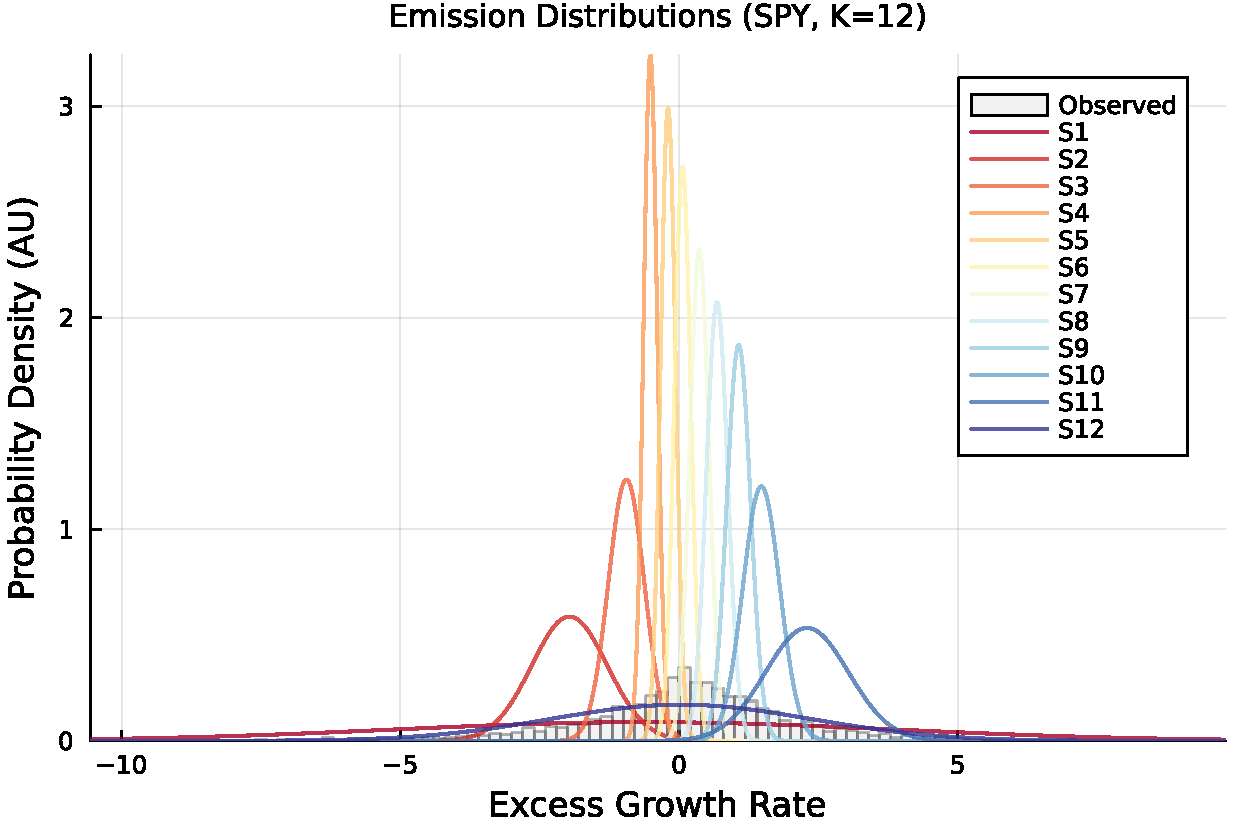
\includegraphics[width=\textwidth]{sections/figs/Fig-Emission-PDFs-K12.pdf}
    \caption{$K = 12$}
\end{subfigure}
\hfill
\begin{subfigure}[b]{0.24\textwidth}
    
\includegraphics[width=\textwidth]{sections/figs/Fig-Emission-PDFs-K18.pdf}
    \caption{$K = 18$ (selected)}
\end{subfigure}
\caption{Learned Gaussian emission distributions across state resolutions, overlaid on the observed SPY return histogram. Higher $K$ values produce finer decomposition with dedicated states capturing tail behavior.}
\label{fig:emissions_all}
\end{figure}

\subsection{Transition Matrix Structure}

Figure~\ref{fig:transition_all} shows the learned transition matrices for $K = 6$ and $K = 18$ in log$_{10}$ color scale.
Both matrices exhibit a dominant near-diagonal band, reflecting the tendency of the market to remain in its current regime.
Off-diagonal entries decay with distance from the diagonal, indicating that large regime jumps (for example, from a deep crash state directly to a boom state) are rare but nonzero.

The diagonal dominance is critical for the ACF-MAE result discussed in Section~\ref{sec:discussion}: the self-transition probabilities $T_{kk}$ for central states are typically 0.7--0.95, producing mean sojourn times of 3--20 days.
The mixture of these geometric sojourn times across states produces the sum-of-exponentials ACF profile that approximates the observed slow decay.

\begin{figure}[H]
\centering
\begin{subfigure}[b]{0.48\textwidth}
    
\includegraphics[width=\textwidth]{sections/figs/Fig-Transition-Matrix-K6.pdf}
    \caption{$K = 6$}
\end{subfigure}
\hfill
\begin{subfigure}[b]{0.48\textwidth}
    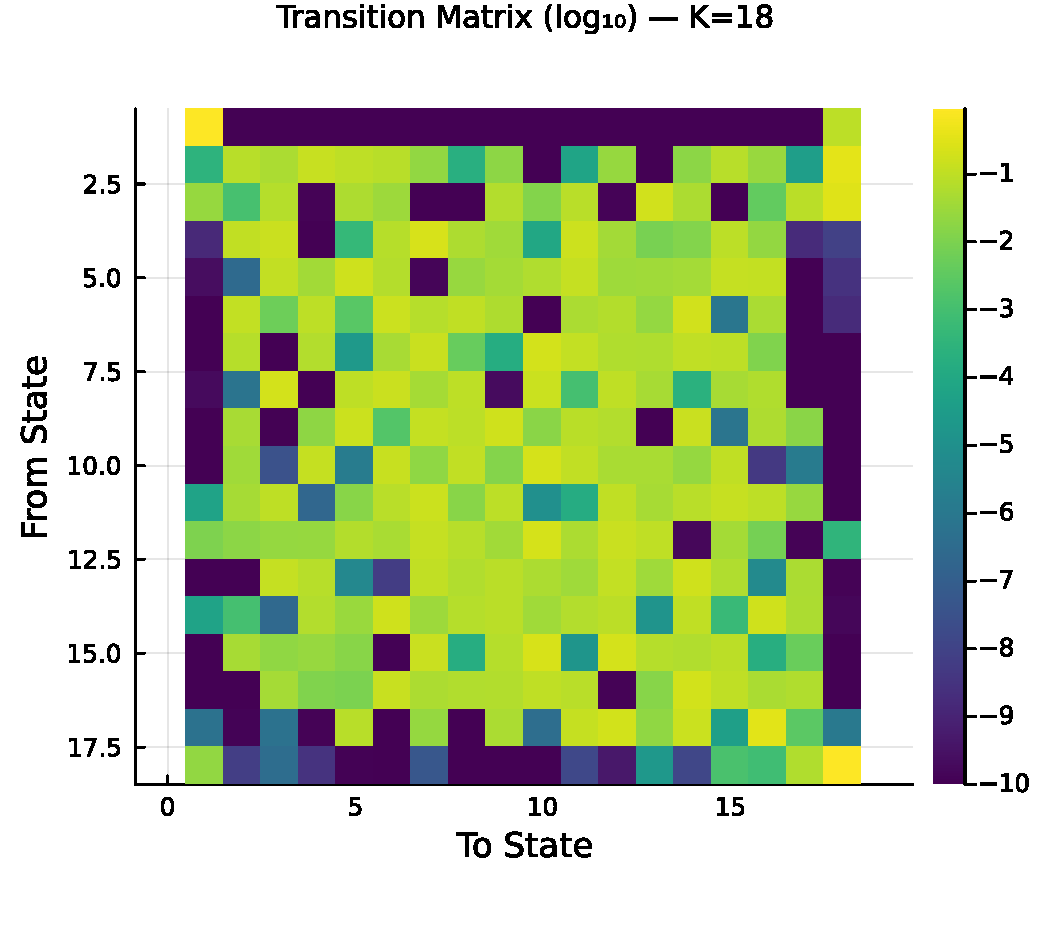
\includegraphics[width=\textwidth]{sections/figs/Fig-Transition-Matrix-K18.pdf}
    \caption{$K = 18$ (selected)}
\end{subfigure}
\caption{Learned transition matrices in log$_{10}$ color scale. The near-diagonal band reflects regime persistence; off-diagonal entries decay with distance, indicating that large regime transitions are rare.}
\label{fig:transition_all}
\end{figure}

\subsection{Stationary Distributions and Residence Times}

Figure~\ref{fig:stationary_all} shows the stationary distributions $\bar{\boldsymbol{\pi}}$ for $K = 6$ and $K = 18$.
In both cases, the central states (those with $\mu_k$ near zero and moderate $\sigma_k$) receive the highest stationary probability, consistent with the empirical concentration of returns near zero.
Tail states (crash and boom) receive low stationary probability, consistent with the rarity of extreme events.

Figure~\ref{fig:residence_all} shows the natural residence times $\tau_k = 1/(1 - T_{kk})$ per state for $K = 6$ and $K = 18$.
Under pure Markov dynamics (no jump mechanism), the expected duration in state $k$ before transitioning is $\tau_k$ steps.
Central states exhibit the longest residence times (5--20 days), while tail states have shorter residence times (1--3 days), consistent with the transient nature of extreme market events.
Notably, even without a jump mechanism, the tail states at higher $K$ maintain sufficient self-transition probability ($T_{kk} \approx 0.3$--$0.5$) to produce multi-day tail episodes.
This contrasts with the discrete model of \citet{alswaidan2026hybrid}, where tail-state residence times were too short to sustain clustering without the Poisson jump extension.

\begin{figure}[H]
\centering
\begin{subfigure}[b]{0.48\textwidth}
    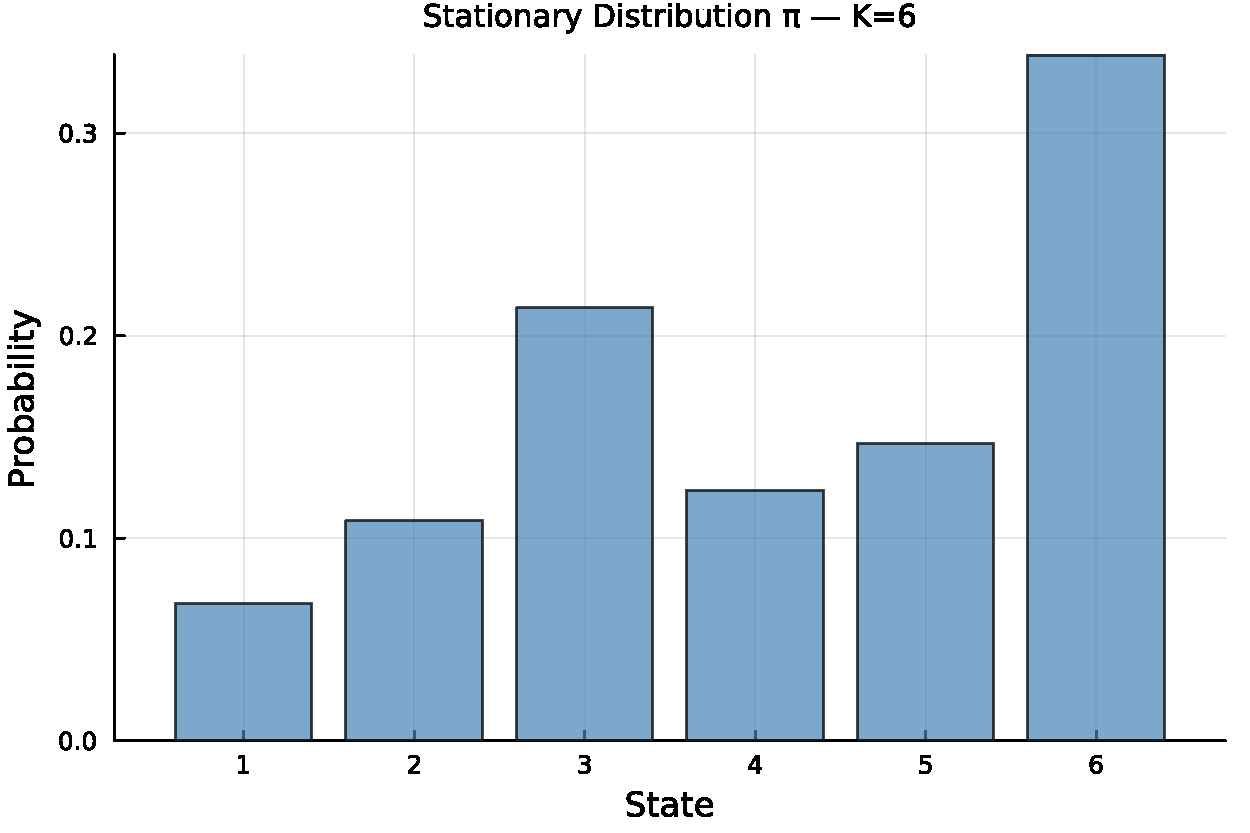
\includegraphics[width=\textwidth]{sections/figs/Fig-Stationary-Distribution-K6.pdf}
    \caption{$K = 6$}
\end{subfigure}
\hfill
\begin{subfigure}[b]{0.48\textwidth}
    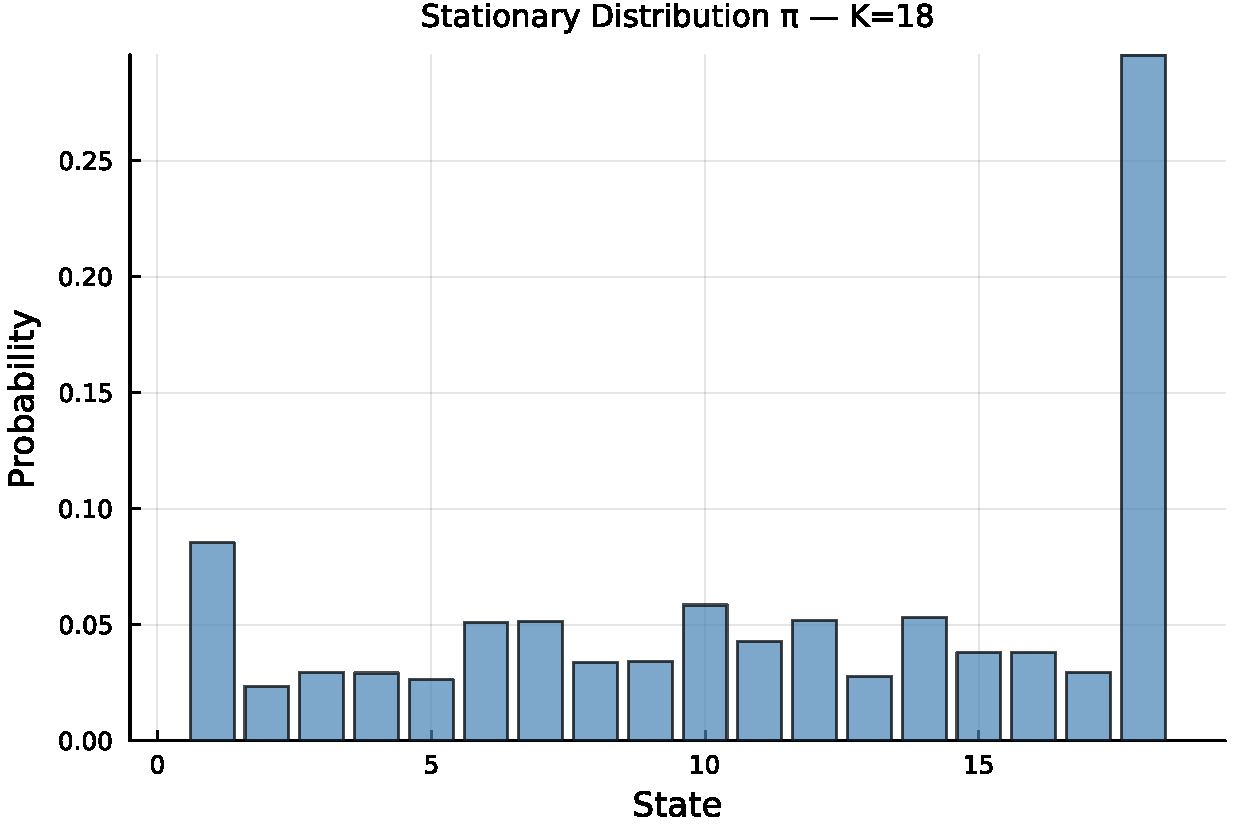
\includegraphics[width=\textwidth]{sections/figs/Fig-Stationary-Distribution-K18.pdf}
    \caption{$K = 18$}
\end{subfigure}
\caption{Stationary distributions $\bar{\boldsymbol{\pi}}$ for $K = 6$ and $K = 18$. Central states receive the highest stationary probability, consistent with the concentration of returns near zero.}
\label{fig:stationary_all}
\end{figure}

\begin{figure}[H]
\centering
\begin{subfigure}[b]{0.48\textwidth}
    
\includegraphics[width=\textwidth]{sections/figs/Fig-Residence-Times-K6.pdf}
    \caption{$K = 6$}
\end{subfigure}
\hfill
\begin{subfigure}[b]{0.48\textwidth}
    
\includegraphics[width=\textwidth]{sections/figs/Fig-Residence-Times-K18.pdf}
    \caption{$K = 18$}
\end{subfigure}
\caption{Natural residence times $\tau_k = 1/(1 - T_{kk})$ per state. Central states have the longest residence times (5--20 days), while tail states are shorter-lived (1--3 days). This asymmetry drives volatility clustering.}
\label{fig:residence_all}
\end{figure}

\subsection{In-Sample Comparison at Non-Selected State Resolutions}
\label{sec:k_sweep_panels}

Figure~\ref{fig:k_sweep_panels_is} shows the in-sample model comparison panels for $K \in \{3, 6, 9, 12, 15, 21\}$, complementing the $K = 18$ comparison in Figure~\ref{fig:is_comparison} of the main text.
Across all resolutions, the CHMM's simulated density closely overlays the observed density, and the ACF of absolute returns tracks the slow decay pattern.
The visible improvement from $K = 3$ to $K = 18$ is concentrated in the tails of the Q-Q panel and the steady-state level of the ACF panel.

\begin{figure}[H]
\centering
\begin{subfigure}[b]{0.32\textwidth}
    
\includegraphics[width=\textwidth]{sections/figs/Fig-3-IS-Comparison-K3.pdf}
    \caption{$K = 3$}
\end{subfigure}
\hfill
\begin{subfigure}[b]{0.32\textwidth}
    
\includegraphics[width=\textwidth]{sections/figs/Fig-3-IS-Comparison-K6.pdf}
    \caption{$K = 6$}
\end{subfigure}
\hfill
\begin{subfigure}[b]{0.32\textwidth}
    
\includegraphics[width=\textwidth]{sections/figs/Fig-3-IS-Comparison-K9.pdf}
    \caption{$K = 9$}
\end{subfigure}

\vspace{0.4cm}

\begin{subfigure}[b]{0.32\textwidth}
    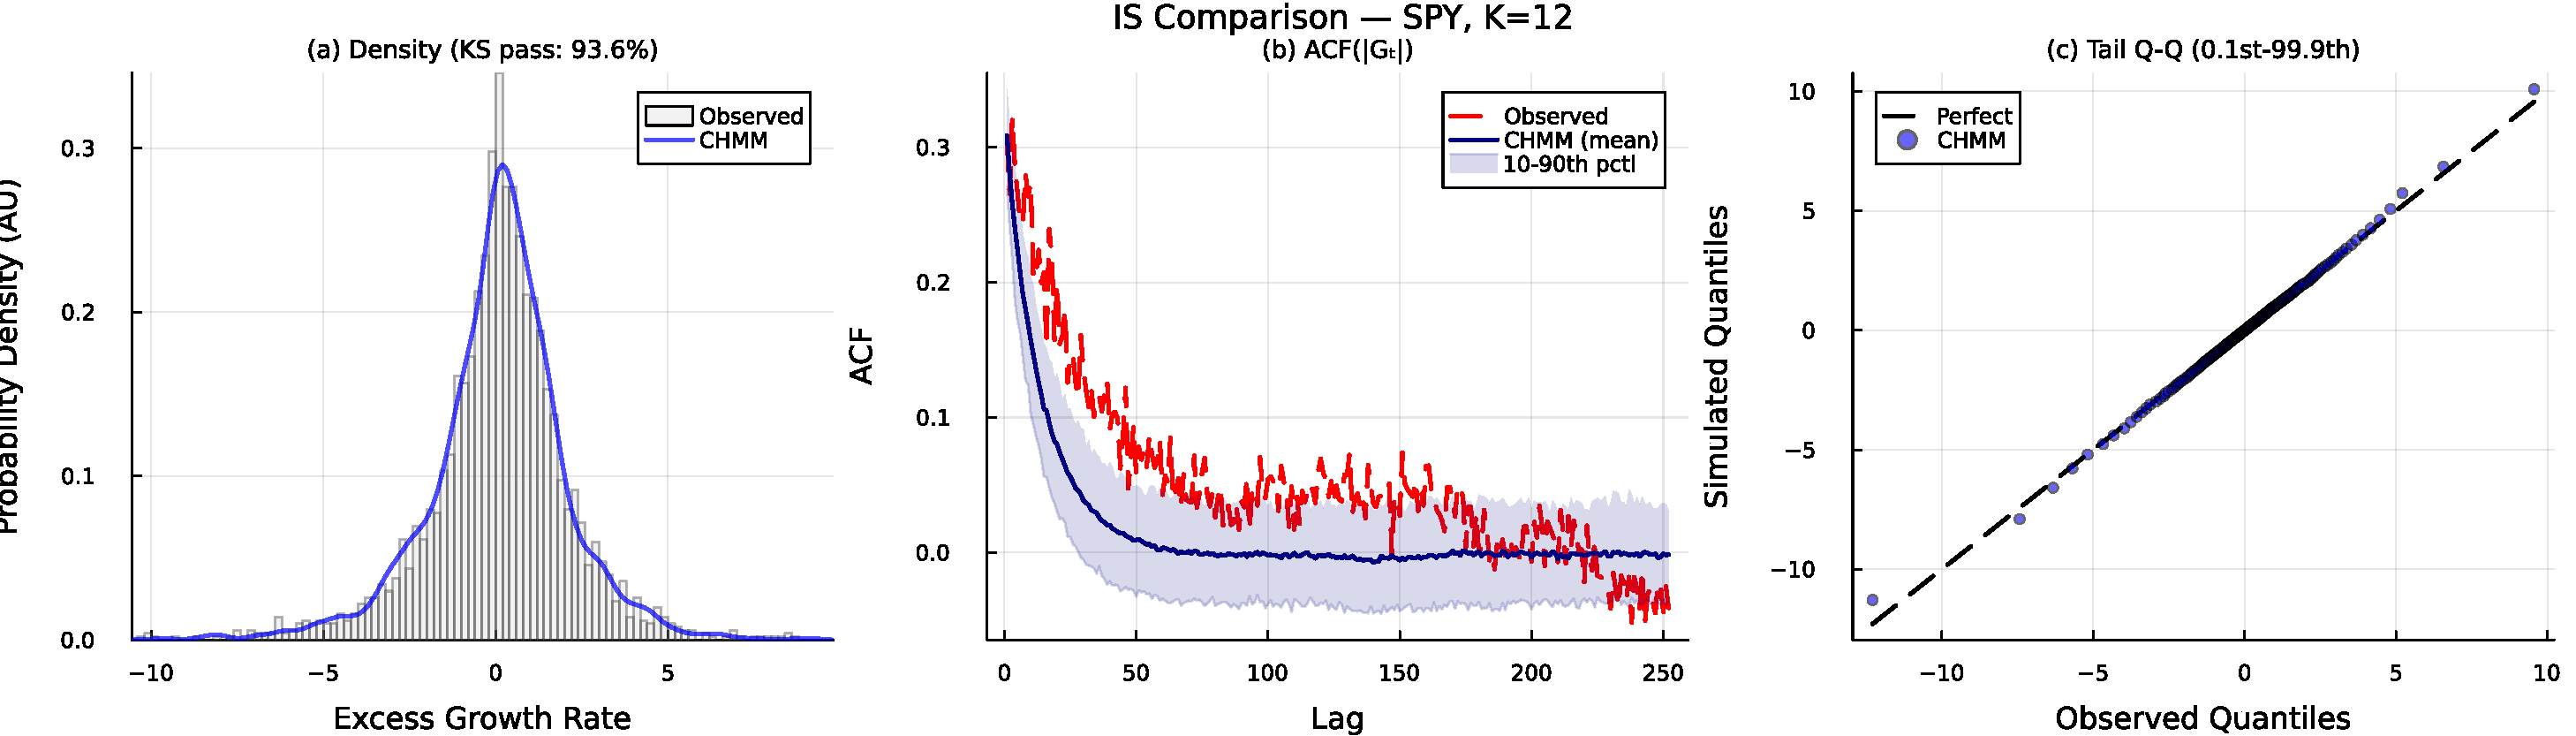
\includegraphics[width=\textwidth]{sections/figs/Fig-3-IS-Comparison-K12.pdf}
    \caption{$K = 12$}
\end{subfigure}
\hfill
\begin{subfigure}[b]{0.32\textwidth}
    
\includegraphics[width=\textwidth]{sections/figs/Fig-3-IS-Comparison-K15.pdf}
    \caption{$K = 15$}
\end{subfigure}
\hfill
\begin{subfigure}[b]{0.32\textwidth}
    
\includegraphics[width=\textwidth]{sections/figs/Fig-3-IS-Comparison-K21.pdf}
    \caption{$K = 21$}
\end{subfigure}
\caption{In-sample CHMM comparison panels at the non-selected state resolutions. Panel $K = 18$ is reproduced in Figure~\ref{fig:is_comparison} of the main text.}
\label{fig:k_sweep_panels_is}
\end{figure}

\subsection{Out-of-Sample Validation at Non-Selected State Resolutions}

Figure~\ref{fig:k_sweep_panels_oos} shows the out-of-sample validation panels for $K \in \{3, 6, 9, 12, 15, 21\}$.
KS pass rates remain above 91\% at all resolutions; the $K = 18$ panel is reproduced in Figure~\ref{fig:oos_validation} of the main text.

\begin{figure}[H]
\centering
\begin{subfigure}[b]{0.32\textwidth}
    
\includegraphics[width=\textwidth]{sections/figs/Fig-4-OoS-Validation-K3.pdf}
    \caption{$K = 3$}
\end{subfigure}
\hfill
\begin{subfigure}[b]{0.32\textwidth}
    
\includegraphics[width=\textwidth]{sections/figs/Fig-4-OoS-Validation-K6.pdf}
    \caption{$K = 6$}
\end{subfigure}
\hfill
\begin{subfigure}[b]{0.32\textwidth}
    
\includegraphics[width=\textwidth]{sections/figs/Fig-4-OoS-Validation-K9.pdf}
    \caption{$K = 9$}
\end{subfigure}

\vspace{0.4cm}

\begin{subfigure}[b]{0.32\textwidth}
    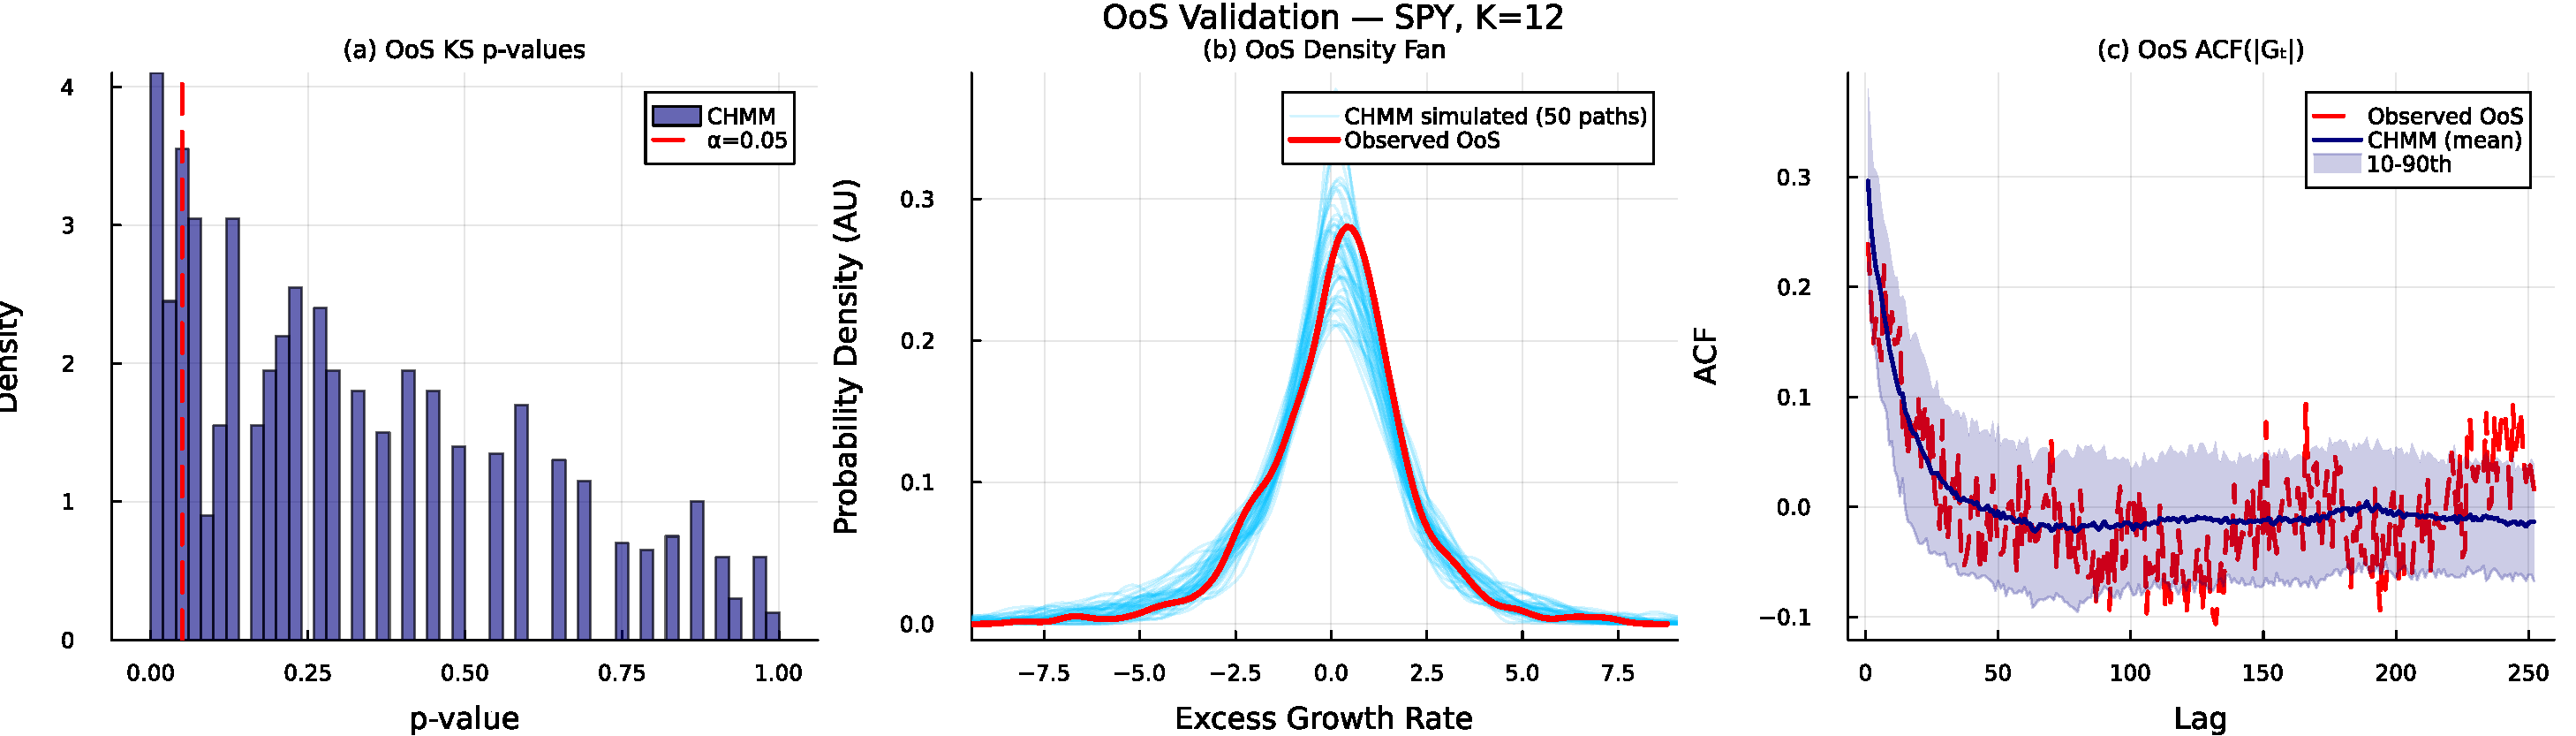
\includegraphics[width=\textwidth]{sections/figs/Fig-4-OoS-Validation-K12.pdf}
    \caption{$K = 12$}
\end{subfigure}
\hfill
\begin{subfigure}[b]{0.32\textwidth}
    
\includegraphics[width=\textwidth]{sections/figs/Fig-4-OoS-Validation-K15.pdf}
    \caption{$K = 15$}
\end{subfigure}
\hfill
\begin{subfigure}[b]{0.32\textwidth}
    
\includegraphics[width=\textwidth]{sections/figs/Fig-4-OoS-Validation-K21.pdf}
    \caption{$K = 21$}
\end{subfigure}
\caption{Out-of-sample CHMM validation panels at the non-selected state resolutions.}
\label{fig:k_sweep_panels_oos}
\end{figure}

\subsection{ACF Comparison Across State Resolutions}

Figure~\ref{fig:acf_all} shows the ACF of $|G_t|$ for the CHMM at $K = 3$, $K = 12$, and $K = 18$, compared to the observed ACF.
At all resolutions, the simulated ACF (shown as the median with 10th--90th percentile envelope across 1{,}000 paths) tracks the observed slow decay pattern.

\begin{figure}[H]
\centering
\begin{subfigure}[b]{0.32\textwidth}
    
\includegraphics[width=\textwidth]{sections/figs/Fig-ACF-Comparison-K3.pdf}
    \caption{$K = 3$}
\end{subfigure}
\hfill
\begin{subfigure}[b]{0.32\textwidth}
    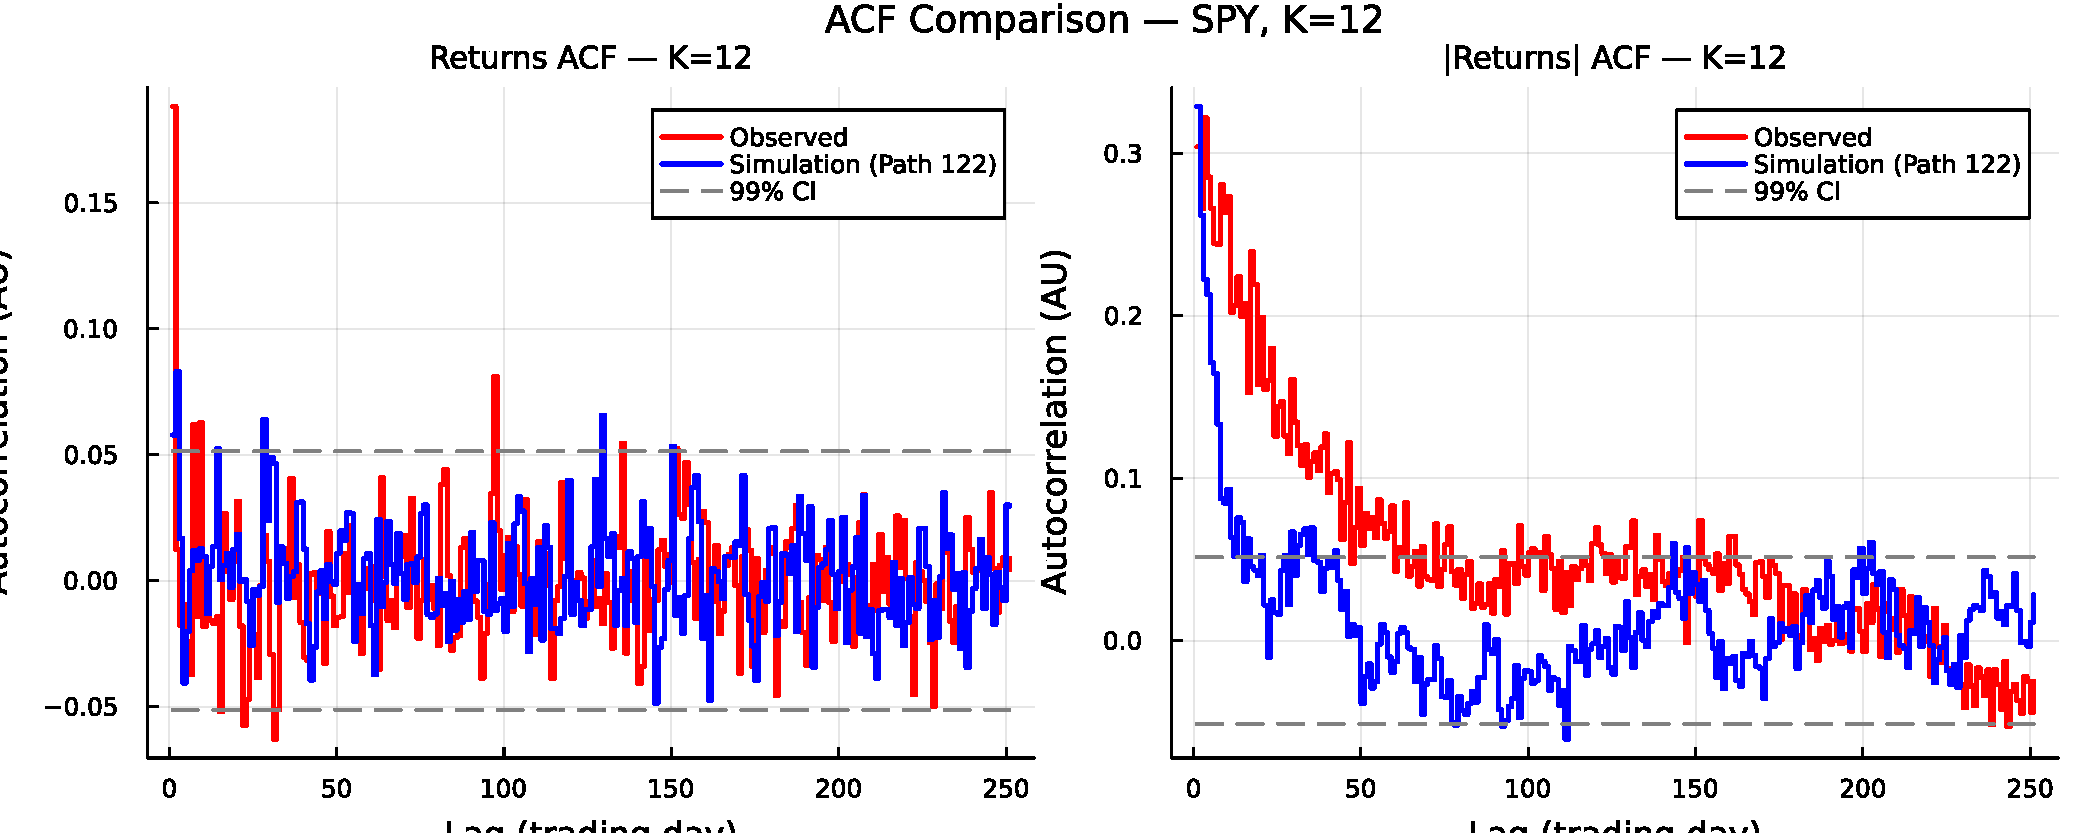
\includegraphics[width=\textwidth]{sections/figs/Fig-ACF-Comparison-K12.pdf}
    \caption{$K = 12$}
\end{subfigure}
\hfill
\begin{subfigure}[b]{0.32\textwidth}
    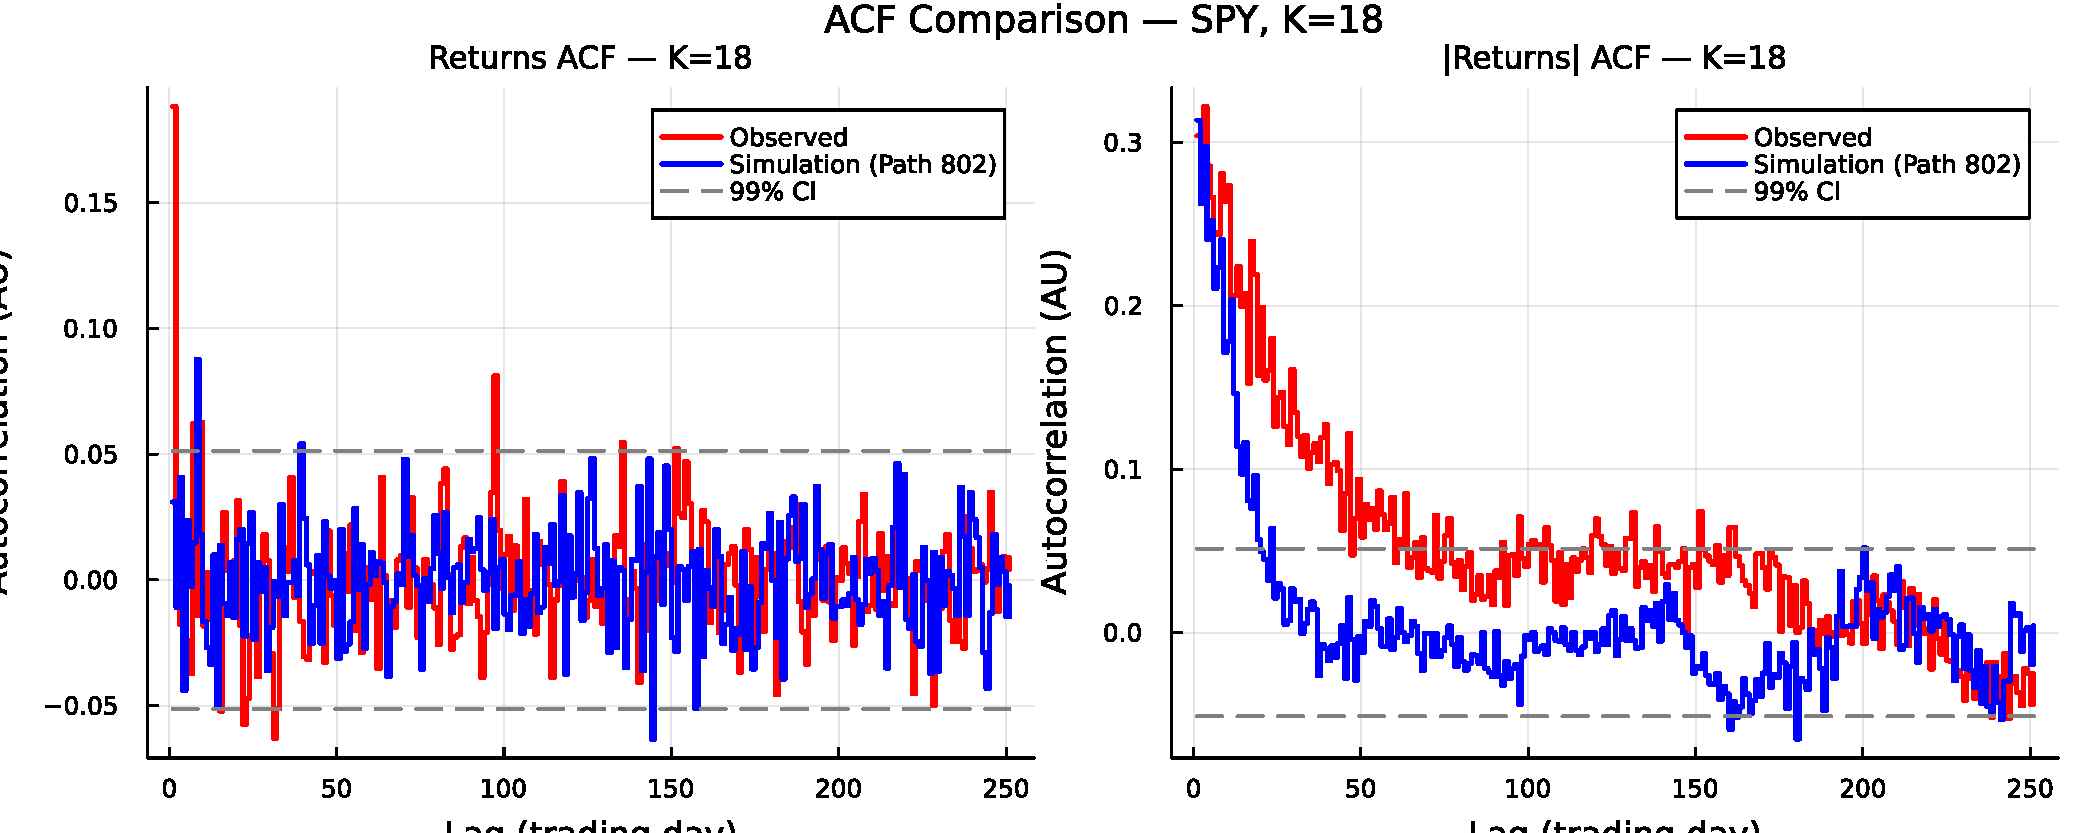
\includegraphics[width=\textwidth]{sections/figs/Fig-ACF-Comparison-K18.pdf}
    \caption{$K = 18$ (selected)}
\end{subfigure}
\caption{ACF of $|G_t|$ for the CHMM at $K = 3$, $K = 12$, and $K = 18$. The simulated 10th--90th percentile envelope (shaded) envelopes the observed ACF (red dashed), confirming that the CHMM reproduces volatility clustering without jump augmentation across the entire sweep.}
\label{fig:acf_all}
\end{figure}

\subsection{Example Simulated Trajectories}

Figure~\ref{fig:trajectories} shows example simulated return trajectories for $K = 6$ and $K = 18$, illustrating the qualitative dynamics produced by the CHMM.
Both trajectories exhibit the characteristic pattern of financial returns: extended periods of low volatility punctuated by clusters of large-magnitude events.

\begin{figure}[H]
\centering
\begin{subfigure}[b]{0.48\textwidth}
    
\includegraphics[width=\textwidth]{sections/figs/Fig-Trajectory-Example-K6.pdf}
    \caption{$K = 6$}
\end{subfigure}
\hfill
\begin{subfigure}[b]{0.48\textwidth}
    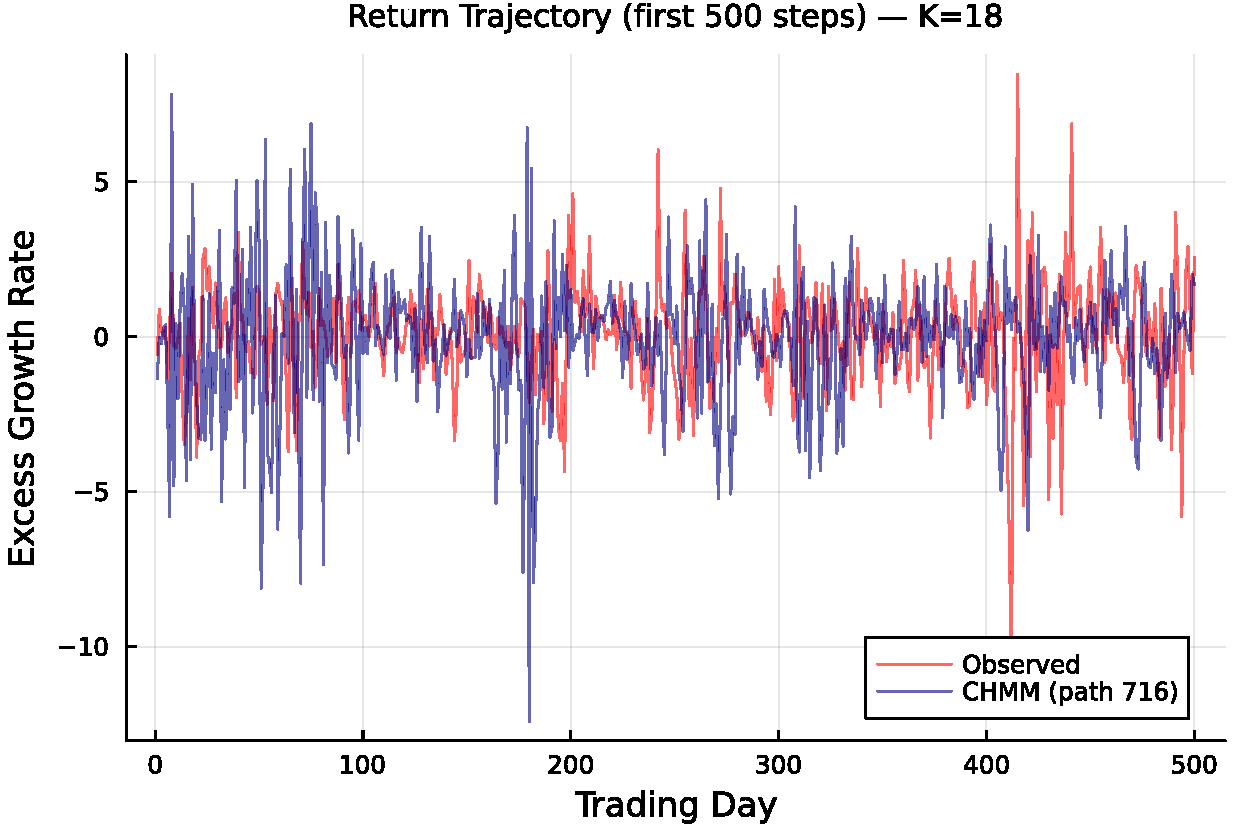
\includegraphics[width=\textwidth]{sections/figs/Fig-Trajectory-Example-K18.pdf}
    \caption{$K = 18$}
\end{subfigure}
\caption{Example simulated return trajectories. The alternation between calm (central states) and volatile (tail states) periods produces the volatility clustering characteristic of empirical financial returns.}
\label{fig:trajectories}
\end{figure}

\subsection{Cross-Asset Dependence Models: Derivations and Diagnostics}
\label{sec:cross_asset_supp}

This appendix provides the technical background for the SIM and copula constructions used in Section~\ref{sec:cross_asset} of the main text.

\paragraph{Sklar's theorem and the rank-reordering simulator.}
Sklar's theorem \cite{sklar1959fonctions, nelsen2006introduction} states that any $d$-dimensional joint CDF $H(g_1, \dots, g_d)$ with continuous marginals $F_1, \dots, F_d$ can be written as $H = C(F_1, \dots, F_d)$ for a unique copula $C$.
The rank-reordering simulator exploits this uniqueness.
If $\tilde{\mathbf{G}}$ is a matrix whose $j$-th column is an i.i.d.\ sample from $F_j$, and $\mathbf{U}$ is an independent sample from $C$, then reordering each column of $\tilde{\mathbf{G}}$ so that its ranks match $\mathbf{U}$'s produces a sample from $H$, up to discrete approximation error in the empirical ranks.
Crucially, reordering never creates new values: each column of the output is a permutation of the corresponding column of $\tilde{\mathbf{G}}$, so marginal distributions are preserved exactly \cite{iman1982distribution}.

\paragraph{Kendall's $\tau$ inversion.}
Given in-sample returns $\mathbf{R} \in \mathbb{R}^{T \times d}$, we estimate the pairwise Kendall's $\tau_{ij}$ from concordant/discordant pair counts and invert to the correlation scale via the analytic relationship $\rho_{ij} = \sin(\pi \tau_{ij} / 2)$, which holds exactly for the Gaussian copula family and is commonly used as a robust correlation estimator for the Student-t copula \cite{embrechts2002correlation, mcneil2015quantitative}.
The resulting matrix $\hat{\Sigma}$ is symmetric but not guaranteed positive semi-definite; we project to the nearest PSD matrix by clipping negative eigenvalues to $10^{-8}$ and rescaling the diagonal to unity.

\paragraph{Profile MLE for $\nu$.}
The Student-t copula log-density at a single pseudo-uniform observation $\mathbf{u} \in [0,1]^d$ is
\begin{equation}
  \log c_t(\mathbf{u}; \Sigma, \nu) \;=\; \log \Gamma\!\left(\tfrac{\nu+d}{2}\right) + (d-1)\log \Gamma\!\left(\tfrac{\nu}{2}\right) - d \log \Gamma\!\left(\tfrac{\nu+1}{2}\right) - \tfrac{1}{2} \log |\Sigma|
  - \tfrac{\nu+d}{2} \log\!\left(1 + \tfrac{\mathbf{x}^\top \Sigma^{-1} \mathbf{x}}{\nu}\right) + \sum_{j=1}^d \tfrac{\nu+1}{2} \log\!\left(1 + \tfrac{x_j^2}{\nu}\right),
  \label{eq:tcop_ll}
\end{equation}
where $x_j = t_\nu^{-1}(u_j)$.
Summing over $t = 1, \dots, T$ pseudo-observations yields the profile log-likelihood as a function of $\nu$ with $\Sigma$ held fixed at the Kendall's-$\tau$ estimate.
We evaluate equation~\eqref{eq:tcop_ll} on the discrete grid $\nu \in \{2, 3, 4, 5, 6, 8, 10, 15, 20, 30\}$ and select $\hat{\nu}$ as the grid point with the largest total log-likelihood.
In Section~\ref{sec:cross_asset} the selected value was $\hat{\nu} = 6$ on the six-asset universe.

\paragraph{Sampling the copula.}
To sample $T$ rows from the $d$-dimensional Gaussian copula with correlation $\Sigma$, we (i) compute the Cholesky factor $\Sigma = L L^\top$, (ii) draw $Z \sim \mathcal{N}(0, I_d)$ i.i.d.\ and form $Y = L Z$, and (iii) return $U = \Phi(Y)$ componentwise.
For the Student-t copula with degrees of freedom $\nu$, we draw $W \sim \chi^2_\nu / \nu$ independent of $Y$ and form the multivariate-$t$ variate $X = Y / \sqrt{W}$, then return $U = t_\nu(X)$ componentwise.

\paragraph{SIM regression summary.}
Table~\ref{tab:sim_regression} reports the fitted SIM regression coefficients and goodness-of-fit statistics for the non-market assets in Section~\ref{sec:cross_asset}.
QQQ's high $R^2 = 0.841$ reflects that the Nasdaq-100 ETF is essentially a linear combination of large-cap technology names that also drive the S\&P~500 index, while JNJ's lower $R^2 = 0.225$ reflects the limited systematic exposure of low-beta healthcare stocks.
These factor loadings and residual magnitudes are what the SIM simulation in equation~\eqref{eq:sim_sim} re-injects at simulation time, and they explain the uneven per-asset KS pass rates reported in Table~\ref{tab:cross_asset_sim_copula}.

\begin{table}[H]
\centering
\caption{SIM regression $\hat{G}_{j,t} = \hat{\alpha}_j + \hat{\beta}_j G_{\text{SPY},t} + \hat{\eta}_{j,t}$ for the five non-market assets, fitted on the 2014--2024 in-sample window ($T = 2{,}766$). Coefficients $\hat{\alpha}, \hat{\beta}$ and $R^2$ are reported for the factor equation used in equation~\eqref{eq:sim_sim}.}
\label{tab:sim_regression}
\small
\begin{tabular}{l ccc}
\toprule
Ticker & $\hat{\alpha}$ & $\hat{\beta}$ & $R^2$ \\
\midrule
NVDA & $0.347$   & $1.749$ & $0.370$ \\
JNJ  & $-0.016$  & $0.539$ & $0.225$ \\
JPM  & $0.001$   & $1.204$ & $0.483$ \\
AAPL & $0.106$   & $1.194$ & $0.474$ \\
QQQ  & $0.041$   & $1.134$ & $0.841$ \\
\bottomrule
\end{tabular}
\end{table}

\subsection{VIX Results Detail}

The CHMM framework was applied to VIX daily log returns to test generalization beyond equity returns.
VIX returns exhibit positive skewness (reflecting asymmetric volatility spikes), pronounced mean reversion, and extreme excess kurtosis, properties that differ fundamentally from equity returns.

The CHMM captured these properties effectively: at higher state resolutions ($K \geq 9$), the model achieved IS KS pass rates above 99\%, demonstrating that the Gaussian mixture mechanism can approximate even the positively skewed, heavy-tailed marginal distribution of VIX returns.
The regime decomposition provided by the Viterbi algorithm aligned with known market events, assigning high-volatility states to crisis episodes and low-volatility states to calm market periods.

The VIX extension demonstrates that the CHMM framework is not limited to equity returns but applies more broadly to financial time series with regime-switching dynamics.
The decoded regimes and their associated median VIX levels provide the volatility map described in Section~\ref{sec:vix_methods}, linking the statistical model to the regime-switching GBM simulation.

\subsection{Algorithm Descriptions}
\label{sec:algorithms}

This section provides detailed pseudocode for the main algorithms used in this study.
Algorithm~\ref{alg:baum_welch} describes the Baum-Welch (EM) procedure for learning CHMM parameters from continuous observations.
Algorithm~\ref{alg:viterbi} presents the Viterbi algorithm for decoding the most likely hidden state sequence.
Algorithm~\ref{alg:chmm_simulate} describes the CHMM simulation procedure for generating synthetic return paths.
Algorithm~\ref{alg:copula_sim} describes the cross-asset rank-reordering simulator for copula-based multi-asset synthesis.
Algorithm~\ref{alg:sim_build} details the SIM regression-and-resampling pipeline.

% ========================================================================================= %
% Algorithm 1: Baum-Welch (EM) for Continuous Gaussian HMM
% ========================================================================================= %
\begin{algorithm}[tp]
\caption{Baum-Welch (EM) algorithm for continuous Gaussian HMM parameter estimation}
\label{alg:baum_welch}
\small
\begin{algorithmic}[1]
\REQUIRE Observations $O_{1:T}$, Number of states $K$, Tolerance $\text{tol}$, Max iterations $\texttt{max\_iter}$
\ENSURE Transition matrix $\mathbf{T}$, Emission parameters $\{\mu_k, \sigma_k\}_{k=1}^K$, Initial distribution $\boldsymbol{\pi}$, Log-likelihood history

\STATE \textbf{Quantile-Based Initialization.}
\STATE Sort observations: $O^{(\text{sort})} \leftarrow \text{sort}(O_{1:T})$.
\STATE Partition $O^{(\text{sort})}$ into $K$ equal-sized chunks $\{C_1, \ldots, C_K\}$.
\FOR{$k = 1$ to $K$}
    \STATE $\mu_k \leftarrow \text{mean}(C_k)$, \quad $\sigma_k \leftarrow \max(\text{std}(C_k),\; 10^{-6})$.
\ENDFOR
\STATE $T_{ij} \leftarrow 1/K$ for all $i, j$; \quad $\pi_k \leftarrow 1/K$ for all $k$.
\STATE $\mathcal{L}_{\text{prev}} \leftarrow -\infty$.

\STATE \textbf{EM Loop.}
\FOR{$n = 1$ to $\texttt{max\_iter}$}

    \STATE \textbf{E-Step:} Compute emission log-likelihoods $\log B_{t,k} = \log \mathcal{N}(O_t \mid \mu_k, \sigma_k^2)$ for all $t, k$.

    \STATE \textit{Forward pass:}
    \STATE $\log \alpha_1(k) \leftarrow \log \pi_k + \log B_{1,k}$ for all $k$.
    \FOR{$t = 2$ to $T$}
        \FOR{$j = 1$ to $K$}
            \STATE $\log \alpha_t(j) \leftarrow \underset{i}{\text{logsumexp}}\!\left(\log \alpha_{t-1}(i) + \log T_{ij}\right) + \log B_{t,j}$
        \ENDFOR
    \ENDFOR

    \STATE \textit{Backward pass:}
    \STATE $\log \beta_T(k) \leftarrow 0$ for all $k$.
    \FOR{$t = T-1$ down to $1$}
        \FOR{$i = 1$ to $K$}
            \STATE $\log \beta_t(i) \leftarrow \underset{j}{\text{logsumexp}}\!\left(\log T_{ij} + \log B_{t+1,j} + \log \beta_{t+1}(j)\right)$
        \ENDFOR
    \ENDFOR

    \STATE \textit{Posterior quantities:}
    \FOR{$t = 1$ to $T$}
        \STATE $\gamma_t(k) \leftarrow \exp\!\left(\log \alpha_t(k) + \log \beta_t(k) - \underset{j}{\text{logsumexp}}(\log \alpha_t(j) + \log \beta_t(j))\right)$ for all $k$.
    \ENDFOR
    \FOR{$t = 1$ to $T-1$}
        \FOR{$i = 1$ to $K$}
            \FOR{$j = 1$ to $K$}
                \STATE $\xi_t(i,j) \leftarrow \exp\!\left(\log \alpha_t(i) + \log T_{ij} + \log B_{t+1,j} + \log \beta_{t+1}(j) - \text{norm}\right)$
            \ENDFOR
        \ENDFOR
    \ENDFOR

    \STATE \textbf{M-Step:} Re-estimate parameters.
    \STATE $\pi_k \leftarrow \gamma_1(k)$ for all $k$.
    \FOR{$k = 1$ to $K$}
        \STATE $\mu_k \leftarrow \sum_{t=1}^T \gamma_t(k) \cdot O_t \;/\; \sum_{t=1}^T \gamma_t(k)$
        \STATE $\sigma_k \leftarrow \max\!\left(\sqrt{\sum_{t=1}^T \gamma_t(k) \cdot (O_t - \mu_k)^2 \;/\; \sum_{t=1}^T \gamma_t(k)},\; 10^{-6}\right)$
    \ENDFOR
    \FOR{$i = 1$ to $K$}
        \STATE $T_{i,j} \leftarrow \sum_{t=1}^{T-1} \xi_t(i,j) \;/\; \sum_{t=1}^{T-1} \gamma_t(i)$ for all $j$.
    \ENDFOR

    \STATE \textbf{Convergence check.}
    \STATE $\mathcal{L}^{(n)} \leftarrow \underset{k}{\text{logsumexp}}(\log \alpha_T(k))$.
    \IF{$|\mathcal{L}^{(n)} - \mathcal{L}_{\text{prev}}| < \text{tol}$}
        \STATE \textbf{break}
    \ENDIF
    \STATE $\mathcal{L}_{\text{prev}} \leftarrow \mathcal{L}^{(n)}$.
\ENDFOR

\RETURN $\mathbf{T}, \{\mu_k, \sigma_k\}_{k=1}^K, \boldsymbol{\pi}$
\end{algorithmic}
\end{algorithm}

% ========================================================================================= %
% Algorithm 2: Viterbi Decoding
% ========================================================================================= %
\begin{algorithm}[tp]
\caption{Viterbi decoding for the most likely hidden state sequence}
\label{alg:viterbi}
\small
\begin{algorithmic}[1]
\REQUIRE Observations $O_{1:T}$, Trained CHMM $\mathcal{M} = (\mathbf{T}, \{\mu_k, \sigma_k\}, \boldsymbol{\pi})$
\ENSURE Most probable state sequence $S_{1:T}^*$

\FOR{$k = 1$ to $K$}
    \STATE $\log \delta_1(k) \leftarrow \log(1/K) + \log \mathcal{N}(O_1 \mid \mu_k, \sigma_k^2)$.
\ENDFOR

\FOR{$t = 2$ to $T$}
    \FOR{$j = 1$ to $K$}
        \STATE $\text{vals}(i) \leftarrow \log \delta_{t-1}(i) + \log T_{ij}$ for all $i$.
        \STATE $\log \delta_t(j) \leftarrow \max_i \text{vals}(i) + \log \mathcal{N}(O_t \mid \mu_j, \sigma_j^2)$.
        \STATE $\psi_t(j) \leftarrow \arg\max_i \text{vals}(i)$.
    \ENDFOR
\ENDFOR

\STATE $S_T^* \leftarrow \arg\max_k \log \delta_T(k)$.
\FOR{$t = T-1$ down to $1$}
    \STATE $S_t^* \leftarrow \psi_{t+1}(S_{t+1}^*)$.
\ENDFOR

\RETURN $S_{1:T}^*$
\end{algorithmic}
\end{algorithm}

% ========================================================================================= %
% Algorithm 3: CHMM Simulation
% ========================================================================================= %
\begin{algorithm}[tp]
\caption{CHMM simulation of synthetic excess growth rate paths}
\label{alg:chmm_simulate}
\small
\begin{algorithmic}[1]
\REQUIRE Trained CHMM $\mathcal{M} = (\mathbf{T}, \{\mu_k, \sigma_k\}, \boldsymbol{\pi})$, Number of steps $M$, Number of paths $P$
\ENSURE Simulated return paths $\{\hat{G}^{(p)}_{1:M}\}_{p=1}^{P}$

\FOR{$p = 1$ to $P$}
    \STATE Sample initial state $S_1 \sim \text{Categorical}(\boldsymbol{\pi})$.
    \FOR{$t = 1$ to $M$}
        \STATE Emit observation $\hat{G}_t^{(p)} \sim \mathcal{N}(\mu_{S_t}, \sigma_{S_t}^2)$.
        \IF{$t < M$}
            \STATE Transition to next state $S_{t+1} \sim \text{Categorical}(\mathbf{T}_{S_t, \cdot})$.
        \ENDIF
    \ENDFOR
\ENDFOR

\RETURN $\{\hat{G}^{(p)}_{1:M}\}_{p=1}^{P}$
\end{algorithmic}
\end{algorithm}

% ========================================================================================= %
% Algorithm 4: Cross-Asset Copula Rank Reordering Simulation
% ========================================================================================= %
\begin{algorithm}[tp]
\caption{Cross-asset copula simulation via rank reordering}
\label{alg:copula_sim}
\small
\begin{algorithmic}[1]
\REQUIRE Fitted per-asset CHMMs $\{\mathcal{M}_j\}_{j=1}^d$, correlation matrix $\Sigma$ (PSD, unit diagonal), copula family $\mathcal{C} \in \{\text{Gaussian}, t_\nu\}$, path length $T$, number of paths $P$
\ENSURE Cross-asset path tensor $\{\hat{G}^{(p)}_{j,t}\}$ of shape $T \times d \times P$

\FOR{$p = 1$ to $P$}

    \STATE Draw copula sample $\mathbf{U}^{(p)} \in [0,1]^{T \times d}$ from $\mathcal{C}(\Sigma)$:
    \STATE \quad $L \leftarrow \text{Cholesky}(\Sigma)$, \; $Z \in \mathbb{R}^{T \times d} \sim \mathcal{N}(0, I_d)$ i.i.d.
    \STATE \quad $Y \leftarrow Z L^\top$
    \IF{$\mathcal{C} = $ Gaussian}
        \STATE \quad $\mathbf{U}^{(p)} \leftarrow \Phi(Y)$ componentwise
    \ELSE
        \STATE \quad Draw $W \sim \chi^2_\nu / \nu$ i.i.d. for $t = 1, \dots, T$; \; $X_{t,\cdot} \leftarrow Y_{t,\cdot} / \sqrt{W_t}$
        \STATE \quad $\mathbf{U}^{(p)} \leftarrow t_\nu(X)$ componentwise
    \ENDIF

    \FOR{$j = 1$ to $d$}
        \STATE Simulate $\tilde{g}_{j,1:T}^{(p)}$ from $\mathcal{M}_j$ via Algorithm~\ref{alg:chmm_simulate}.
        \STATE Compute order statistics $\tilde{g}_{j,(1)}^{(p)} \leq \cdots \leq \tilde{g}_{j,(T)}^{(p)}$.
        \STATE Compute ranks $r_{j,t}^{(p)} \leftarrow \text{rank}(U_{j,t}^{(p)})$ for $t = 1, \dots, T$.
        \STATE $\hat{G}_{j,t}^{(p)} \leftarrow \tilde{g}_{j,(r_{j,t}^{(p)})}^{(p)}$ for $t = 1, \dots, T$.
    \ENDFOR
\ENDFOR

\RETURN $\{\hat{G}^{(p)}_{j,t}\}$
\end{algorithmic}
\end{algorithm}

% ========================================================================================= %
% Algorithm 5: SIM fit and simulate
% ========================================================================================= %
\begin{algorithm}[tp]
\caption{Single Index Model (SIM) construction and simulation}
\label{alg:sim_build}
\small
\begin{algorithmic}[1]
\REQUIRE In-sample return matrix $\mathbf{R} \in \mathbb{R}^{T \times d}$, market-column index $m$, market CHMM $\mathcal{M}_m$, path length $T$, number of paths $P$
\ENSURE Cross-asset path tensor $\{\hat{G}^{(p)}_{j,t}\}$ of shape $T \times d \times P$

\STATE \textbf{OLS fit.} For $j \neq m$:
\STATE \quad $\hat{\beta}_j \leftarrow \text{Cov}(\mathbf{R}_{:,j}, \mathbf{R}_{:,m}) / \text{Var}(\mathbf{R}_{:,m})$
\STATE \quad $\hat{\alpha}_j \leftarrow \overline{\mathbf{R}_{:,j}} - \hat{\beta}_j \overline{\mathbf{R}_{:,m}}$
\STATE \quad $\hat{\eta}_{j,t} \leftarrow R_{t,j} - \hat{\alpha}_j - \hat{\beta}_j R_{t,m}$, \; $R^2_j \leftarrow 1 - \sum_t \hat{\eta}_{j,t}^2 / \sum_t (R_{t,j} - \overline{\mathbf{R}_{:,j}})^2$

\FOR{$p = 1$ to $P$}
    \STATE Simulate market path $G_{m,1:T}^{(p)}$ from $\mathcal{M}_m$ via Algorithm~\ref{alg:chmm_simulate}.
    \STATE $\hat{G}_{m,t}^{(p)} \leftarrow G_{m,t}^{(p)}$.
    \FOR{$j \neq m$}
        \STATE Draw residual indices $\{\iota_t\}_{t=1}^T \sim \text{Uniform}(\{1, \dots, T\})$.
        \STATE $\hat{G}_{j,t}^{(p)} \leftarrow \hat{\alpha}_j + \hat{\beta}_j G_{m,t}^{(p)} + \hat{\eta}_{j,\iota_t}$.
    \ENDFOR
\ENDFOR

\RETURN $\{\hat{G}^{(p)}_{j,t}\}$
\end{algorithmic}
\end{algorithm}


\end{document}
